%%%%%%%%%%%%%%%%%%%%%%%%%%%%%%%%%%%%%%%%%%%%%%%%%%%%%%%%%%%%%%%%%%%%%%
% Lớp 12 | Ứng dụng đạo hàm để khảo sát hàm số | Sự đồng biến và nghịch biến của hàm số
% Dạng 2D1?1-1: Xét tính đơn điệu của hàm số cho bởi công thức
% Số câu: 69  (sinh tự động bởi tach_cau.py; từ nay thầy sửa trực tiếp file này)
%%%%%%%%%%%%%%%%%%%%%%%%%%%%%%%%%%%%%%%%%%%%%%%%%%%%%%%%%%%%%%%%%%%%%%

%%%%%%%%%%%%%%%% TRẮC NGHIỆM 4 PHƯƠNG ÁN %%%%%%%%%%%%%%%%

% nguồn: Phan1_Lop_12_Dai_so_Chuong_1
\begin{ex}%[2D1N1-1]%[ma:598f9989]
	Giá trị lớn nhất của  hàm số $y=\dfrac{x+1}{x-2}$ trên $\left[-1;0\right]$ là
	\choice 
		{$-\dfrac{1}{2}$} 
		 {$-\dfrac{2}{3}$}
		 {$2$}
		{\True $0$} 
	 \loigiai{
		Hàm số $y=\dfrac{x+1}{x-2}$ xác định và liên tục trên $\left[-1;0\right]$ có 
		$y'=\dfrac{-3}{(x-2)^2}<0, \, \forall x \in \left[-1;0\right] $.  \\
		Suy ra hàm số nghịch biến trên $\left[-1;0\right]$.\\ 
		Do đó $\max \limits_{\left[-1;0\right] } y  = y(-1) = 0$.
	 }
\end{ex}

% nguồn: Phan1_Lop_12_Dai_so_Chuong_1
\begin{ex}%[2D1N1-1]%[ma:5da1e42a]
	Cho hàm  số $y=\log _3\left(x^2-2 x+3\right)$. Hàm số đồng biến trên khoảng nào sau đây?
	 \choice
		 {$(-\infty; 1)$}
		 {$(-1;+\infty)$}
		{$(-\infty;-1)$} 
		 {\True $(1;+\infty)$}
	 \loigiai{
		Tập xác định của hàm số đã cho là $\mathbb{R}$ vì $x^2 -2x +3=(x-1)^2 +2>0$, $\forall x$.\\ 
		 Khi đó $y'=\dfrac{2x-2}{\left(x^{2}-2 x+3\right)\cdot \ln 3}$.\\
		$y' \geq  0 \Leftrightarrow 2x-2 \geq 0 \Leftrightarrow x \geq 1$. Suy ra hàm số đồng biến trên khoảng $(1;+\infty)$.
	 }
\end{ex}

% nguồn: Phan1_Lop_12_Dai_so_Chuong_1
\begin{ex}%[2D1N1-1]%[ma:5fad2ac6]
	Hàm số $y=\dfrac{x-7}{x+4}$ đồng biến  trên khoảng
	\choice 
		{$(-\infty;+\infty)$} 
		{$(-6;0)$} 
		 {\True $(1;4)$}
		{$(-5;1)$} 
	\loigiai{Tập  xác định $\mathscr{D}=\mathbb{R} \setminus \left\{-4\right\}$.\\
		Ta có $y'=\dfrac{11}{(x+4)^2} > 0$, $\forall x\in  \mathscr{D}$.\\
	Vậy hàm số đồng biến trên các khoảng $(-\infty;-4)$ và  $(-4;+\infty)$ và đồng biến trên $(1;4)$.}
\end{ex}

% nguồn: Phan1_Lop_12_Dai_so_Chuong_1
\begin{ex}%[2D1N1-1]%[ma:987f360c]
	Các khoảng đồng biến của hàm số $y=x^4-8x^2-4$  là
	\choice 
		 {$(-\infty;-2)$ và $(2;+\infty)$}
		{$(-2;0)$  và $(0;+\infty)$}
		 {$(-\infty;-2)$ và $(0;2)$}
		{\True $(-2;0)$ và $(2;+\infty)$} 
	\loigiai{Ta  có tập xác định của hàm số là $\mathscr{D}=\mathbb{R}$ và $y'=4x^3-16x$.
		$$y'=0\Leftrightarrow  4x^3-16x=0\Leftrightarrow
		\hoac{&x=0\\ 
		&x=-2\\ 
		 &x=2.}$$
		Khi đó $y'\ge 0\Leftrightarrow 4x^3-16x\ge 0\Leftrightarrow  \hoac{&x\ge 2\\
		&-2\le x\le  0.}$ \\
		 Vậy hàm số đồng biến trên các khoảng $(-2;0)$ và $(2;+\infty)$.
	} 
\end{ex}

% nguồn: Phan1_Lop_12_Dai_so_Chuong_1
\begin{ex}%[2D1N1-1]%[ma:38271202]
	Cho hàm số $y=\dfrac{x+1}{x-3}$. Trong các mệnh đề sau, mệnh đề nào  \textbf{sai}?
	 \choice
		{Hàm số nghịch biến trên từng khoảng xác định của  nó}
		{\True  Hàm số nghịch biến trên tập xác định của nó}
		{Hàm  số nghịch biến trên khoảng $(3;+\infty)$}
		 {Hàm số nghịch biến trên khoảng $(-\infty; 3)$}
	\loigiai{Hàm số đã cho có tập xác định gồm hai khoảng $(-\infty; 3)$ và $(3;+\infty)$ rời nhau nên khẳng định hàm số nghịch biến trên tập xác  định là sai.}
\end{ex}

% nguồn: Phan1_Lop_12_Dai_so_Chuong_1
\begin{ex}%[2D1N1-1]%[ma:73141b32]
	Hàm số $y=x^4-2x^2+1$ nghịch biến  trên các khoảng nào sau đây?
	 \choice
		{\True  $(-\infty;-1)$ và $(0;1)$}
		{$(-\infty;-1)$ và  $(0;+\infty)$}
		{$(-\infty;0)$ và  $(1;+\infty)$}
		 {$(-1;0)$ và $(1;+\infty)$}
	\loigiai{Ta có $y'=4x^3-4x=0\Leftrightarrow \hoac{&x=0\\ 
		&x=-1\\ 
		 &x=1.\\
		}$ \\ 
		 Bảng biến thiên
		\begin{center}
			
\begin{tikzpicture}
				\tkzTabInit[nocadre =  false,lgt = 1,espcl = 2]
					{$x$ /1,$y'$  /1,$y$ /2}{$-\infty$,$-1$,$0$,$1$,$+\infty$}
				 \tkzTabLine{,-,$0$,+,$0$,-,$0$,+}
				\tkzTabVar{+/ $+\infty$,-/ $0$,+/ $1$,-/ $0$,+/ $+\infty$} 
			\end{tikzpicture}
		\end{center}
		Vậy hàm số nghịch biến  trên các khoảng
	$(-\infty;-1)$ và  $( 0;1)$.}
\end{ex}

% nguồn: Phan1_Lop_12_Dai_so_Chuong_1
\begin{ex}%[2D1N1-1]%[ma:41015111]
	Cho hàm số $y=\dfrac{1}{3}x^3-\dfrac{1}{2}x^2-12x-1$.  Mệnh đề nào sau đây đúng?
	\choice 
		{Hàm số nghịch biến trên  khoảng $(-3;+\infty)$}
		{Hàm số đồng biến trên khoảng  $(-\infty;4)$}
		 {Hàm số đồng biến trên khoảng $(-3;4)$}
		{\True Hàm số đồng biến trên khoảng  $(4;+\infty)$}
	 \loigiai{
		Ta có $y'=x^2-x-12=0\Leftrightarrow \hoac{&x=-3\\ 
		 &x=4.}$ \\
		Bảng xét  dấu
		\begin{center}
			
\begin{tikzpicture}
				\tkzTabInit[lgt  = 2,espcl = 2.5]
					 {$x$ /1,$y'$/1}
					{$-\infty$,$-3$,$4$,$+\infty$} 
				 \tkzTabLine{,+,0,-,0,+,}
			\end{tikzpicture}
		\end{center}
		Dựa vào bảng xét dấu ta thấy hàm số đồng biến  trên khoảng $(4;+\infty)$.
	 }
\end{ex}

% nguồn: Phan1_Lop_12_Dai_so_Chuong_1
\begin{ex}%[2D1N1-1]%[ma:b04c189c]
	Hàm số nào dưới đây đồng biến trên $\mathbb{R}$? 
	 \choice
		 {$y=x^2+2x+3$}
		 {\True $y=x^3+x+1$}
		{$y=-x^3-3x$} 
		 {$y=\dfrac{x+1}{x+3}$}
	 \loigiai{
		Xét hàm số $y=x^3+x+1$ có $y'=3x^2+1  \ge 0,\forall x \in \mathbb{R}$.\\
	Do đó hàm số đã cho  đồng biến trên $\mathbb{R}$.}
\end{ex}

% nguồn: Phan1_Lop_12_Dai_so_Chuong_1
\begin{ex}%[2D1N1-1]%[ma:3410019a]
	Hàm số $y = \dfrac{2x+3}{x+1}$ có bao  nhiêu điểm cực trị?
	 \choice
		 {$3$}
		 {$2$}
		{\True  $0$}
		 {$1$}
	 \loigiai{
		Tập xác định $\mathscr{D}  = \mathbb{R} \setminus \{-1\}$. Đạo hàm $y'=\dfrac{-1}{(x+1)^2} <0$, $\forall x \neq -1$.\\
		Khi đó hàm  số luôn nghịch biến trên từng khoảng xác định.\\
		Vậy hàm số đã cho không  có cực trị.
	 }
\end{ex}

% nguồn: Phan1_Lop_12_Dai_so_Chuong_1
\begin{ex}%[2D1H1-1]%[ma:ef7bd910]
	Tìm khoảng nghịch biến của hàm số  $y=f(x)$, biết $f'(x)=(x-3)(x+2)(x+5)^2,\forall x\in \mathbb{R}$.
	 \choice
		 {$(-\infty;-5)$}
		{\True  $(-2;3)$}
		 {$(-5;-2)$}
		{$(3;+\infty)$} 
	 \loigiai{
		Ta có  $f'(x)=(x-3)(x+2)(x+5)^2<0\Leftrightarrow (x-3)(x+2)<0,\, (x\ne -5)\Leftrightarrow x^2-x-6<0\Leftrightarrow -2<x<3$.\\
		Vậy  hàm số nghịch biến trên $(-2;3)$.
	} 
\end{ex}

% nguồn: Phan1_Lop_12_Dai_so_Chuong_1
\begin{ex}%[2D1H1-1]%[ma:ba0ab6fd]
	Hàm số nào  sau đây \textbf{không} đồng biến trên $(-\infty;+\infty)$?
	 \choice
		{$y=x^5+x^3-1$} 
		 {$y=x^3+2$}
		 {\True $y=\dfrac{x-1}{x+2}$}
		 {$y=x+1$}
	 \loigiai{
		Ta có  $y=\dfrac{x-1}{x+2}\Rightarrow y'=\dfrac{3}{{(x+2)}^2} > 0,\forall x\ne-2$. \\
	Do đó hàm số đồng biến trên các khoảng $(-\infty;2)$  và $(2;+\infty)$.}
\end{ex}

% nguồn: Phan1_Lop_12_Dai_so_Chuong_1
\begin{ex}%[2D1H1-1]%[ma:11ba45bd]
	Cho hàm số $y=f(x)$ liên tục  trên $\mathbb{R}$ và có đạo hàm $f'(x)=(x+1)(x-1)^4(2-x)$. Mệnh đề nào dưới đây đúng?
	\choice 
		 {$f(5)>f(4)>f(3)$}
		 {$f(-1)>f(0)>f(1)$}
		 {$f(-3)<f(-2)<f(-1)$}
		{\True $f(0)<f(1)<f(2)$} 
	\loigiai{ 
		\begin{center}
			
\begin{tikzpicture}
				\tkzTabInit 
					 {$x$/1,$f'(x)$/1}
					{$-\infty$,$-1$,$1$,$2$,$+\infty$} 
				 \tkzTabLine{,-,0,+,0,+,0,-,}
			\end{tikzpicture}
		\end{center}
	Vì $f'(x)\geq 0\Leftrightarrow x\in (-1;2)$ nên hàm số đồng biến trên khoảng $(-1;2)$. \\ Do đó,  ta có $f(0)<f(1)<f(2)$.}
\end{ex}

% nguồn: Phan1_Lop_12_Dai_so_Chuong_1
\begin{ex}%[2D1H1-1]%[ma:f5e8887f]
	Cho hàm số $y=\dfrac{8-5x}{-4x-9}$. Khẳng định  nào sau đây là \textbf{sai}?
	 \choice
		{Hàm số  đồng biến trên khoảng $\left(-\infty;-\dfrac{37}{4}\right)$}
		{Hàm số đồng biến trên khoảng $\left(-\infty;-\dfrac{9}{4}\right)$} 
		{Hàm  số đồng biến trên khoảng $\left(-\dfrac{9}{4};+\infty\right)$}
		 {\True Hàm số nghịch biến trên khoảng $\left(-\infty;-\dfrac{37}{4}\right)$}
	 \loigiai{
		Tập xác định  $\mathscr{D}=\mathbb{R}\backslash\left\{-\dfrac{9}{4}\right\}$.\\
		$y'=\dfrac{-5\cdot(-9)-8\cdot(-4)}{\left(-4x-9\right)^{2}}=\dfrac{77}{\left(-4x-9\right)^{2}}>0,\forall x \in \mathscr{D}$.\\ 
		Do đó, hàm  số đồng biến trên mỗi khoảng $\left(-\infty;-\dfrac{9}{4}\right)$ và $\left(-\dfrac{9}{4};+\infty\right)$.
	 }
\end{ex}

% nguồn: Phan1_Lop_12_Dai_so_Chuong_1
\begin{ex}%[2D1H1-1]%[ma:e7d71728]
	Cho hàm số $ y=\dfrac{x-3}{x+1}$. Mệnh đề nào dưới đây đúng? 
	\choice 
		{Hàm số đồng biến trên $\mathbb{R}\setminus\left\{-1\right\}$} 
		{Hàm  số nghịch biến trên $(-\infty;-1)$}
		{Hàm  số đồng biến trên $(-\infty;+\infty)$}
		 {\True Hàm số đồng biến trên $(-\infty;-1)$}
	\loigiai{ 
		Ta có $ y'=\dfrac{4}{(x+1)^2}>0$,  với $x$ thuộc khoảng $(-\infty;-1)$ và $(-1;+\infty)$.\\
	Vậy  hàm số đồng biến trên $(-\infty;-1)$.}
\end{ex}

% nguồn: Phan1_Lop_12_Dai_so_Chuong_1
\begin{ex}%[2D1H1-1]%[ma:e75abc82]
	Cho hàm số $ y=\dfrac{x+2}{x-1}$. Xét các mệnh đề sau: 
	\begin{enumerate}[1)]
		\item Hàm số đã cho đồng biến trên  $(1;+\infty)$.
		\item  Hàm số đã cho nghịch biến trên $\mathbb{R}\setminus\left\{1\right\}$.
		\item Hàm số đã  cho không có điểm cực trị.
		\item Hàm số đã cho nghịch biến trên các  khoảng $(-\infty;1)$ và $(1;+\infty)$.
	\end{enumerate}
	Số các mệnh  đề đúng là
	\choice 
		 {$ 4$}
		 {\True $ 2$}
		{$ 3$} 
		{$ 1$} 
	\loigiai{ 
		Ta có $ y=\dfrac{x+2}{x-1}\Rightarrow y'=\dfrac{-3}{(x-1)^2}<0$, $\forall x\ne 1$ nên  hàm số đã cho không có điểm cực trị, nghịch biến trên các khoảng $(-\infty;1)$ và $(1;+\infty)$.
	} 
\end{ex}

% nguồn: Phan1_Lop_12_Dai_so_Chuong_1
\begin{ex}%[2D1H1-1]%[ma:93e45daa]
	Cho hàm số $y=x-2\sqrt{x}$. Mệnh  đề nào sau đây đúng?
	\choice 
		 {Hàm số nghịch biến trên khoảng $(1;+\infty)$}
		{\True Hàm  số đồng biến trên khoảng $(2;+\infty)$}
		{Hàm số đồng biến  trên khoảng $(0;+\infty)$}
		{Hàm số  nghịch biến trên khoảng $(-\infty;1)$}
	\loigiai{ 
		Tập xác  định $\mathscr{D}=[0;+\infty)$. \\
		Ta có  $y'=1-\dfrac{1}{\sqrt{x}}=\dfrac{\sqrt{x}-1}{\sqrt{x}}$;
		$y'=0\Leftrightarrow \sqrt{x}=1\Leftrightarrow x=1$.\\ 
		Bảng biến thiên 
		\begin{center}
			
\begin{tikzpicture}
				\tkzTabInit[lgt = 1,espcl =  2.5]
					{$x$  /.7,$y'$ /.7,$y$ /2}
					{$0$,$1$,$+\infty$} 
				 \tkzTabLine{,-,$0$,+,}
				\tkzTabVar{+/  $0$,-/ $-1$,+/ $+\infty$}
			\end{tikzpicture}
		\end{center}
		Từ bảng biến thiên suy ra $y' < 0,\forall  x\in (0;1)$ và $y' > 0,\forall x\in (1;+\infty)$.\\
		Vậy hàm số đồng biến trên khoảng $(1;+\infty)$  suy ra hàm số đồng biến trên khoảng $(2;+\infty)$.
	} 
\end{ex}

% nguồn: Phan1_Lop_12_Dai_so_Chuong_1
\begin{ex}%[2D1H1-1]%[ma:8018419d]
	Cho hàm số $y=f(x)$ có đạo hàm $f'(x)=(x+1){(2x-5)^2}$ với mọi $x\in\mathbb{R}$. Hàm  số đã cho nghịch biến trên khoảng nào?
	 \choice
		 {\True $(-\infty;-1)$}
		{$(-1;3)$} 
		{$(-1;+\infty)$} 
		 {$(-3;1)$}
	 \loigiai{
		Ta có $f'(x)=0\Leftrightarrow \hoac{& x=-1\\& x=\dfrac{5}{2}.}$\\ 
		Bảng  xét dấu $f'(x)$
		\begin{center}
			
\begin{tikzpicture}[font=\footnotesize,>=stealth]
			\tikzset{double style/.append style={double distance=1.5pt}}
			 \tkzTabInit[nocadre=false,lgt=1.2,espcl=2.5,deltacl=0.6]
				 {$x$ /0.7,$f'(x)$ /0.6}
				 {$-\infty$,$-1$,$\dfrac{5}{2}$,$+\infty$}
			\tkzTabLine{,-,$0$,+,$0$,+,} 
		\end{tikzpicture}
		\end{center}
	Vậy hàm số nghịch biến trên khoảng $(-\infty;-1)$  .}
\end{ex}

% nguồn: Phan1_Lop_12_Dai_so_Chuong_1
\begin{ex}%[2D1H1-1]%[ma:9c3560a9]
	Hàm số $y=-x^4+2x^2+1$ đồng biến trên khoảng nào  dưới đây?
	\choice 
		{$(0;+\infty)$} 
		{\True  $(-\infty;-1)$}
		{$(1;+\infty)$} 
		 {$(-\infty;0)$}
	 \loigiai{
		 Tập xác định $D=\mathbb{R}$.\\
		 Ta có $y'=-4x^3+4x$ $\Rightarrow y'=0\Leftrightarrow \hoac{
		 & x=0 \\
		&  x=\pm 1.}$\\
		Bảng biến  thiên:
		\begin{center}
			
\begin{tikzpicture}[scale=.8]
				 \tkzTabInit
					{$x$/1,$y' $/1,$y$/3} 
					 {$-\infty$,$-1$,$0$,$1$,$+\infty$}
				 \tkzTabLine{,+,0,-,0,+,0,-,}
				\tkzTabVar{-/$-\infty$,+/$2$,-/$1$,+/$2$,-/$-\infty$} 
			\end{tikzpicture}
		\end{center}
	Từ bảng biến thiên  ta thấy trên khoảng $(-\infty;-1)$ hàm số đồng biến.}
\end{ex}

% nguồn: Phan1_Lop_12_Dai_so_Chuong_1
\begin{ex}%[2D1H1-1]%[ma:641a4100]
	Cho hàm số $y=f(x)$ có đạo hàm $f'(x)=-x+2$ với  mọi $x\in \mathbb{R}$. Hàm số đã cho nghịch biến trên khoảng nào dưới đây?
	\choice 
		 {$(-\infty;+\infty)$}
		{\True $(2;+\infty)$} 
		 {$(-\infty;2)$}
		 {$(0;+\infty)$}
	\loigiai{ 
		Ta có  $f'(x)=-x+2=0\Leftrightarrow x=2$.\\
		Bảng xét  dấu
		\begin{center}
			
\begin{tikzpicture}
				\tkzTabInit 
					{$x$/1,$f'(x)$/1} 
					 {$-\infty$,$2$,$+\infty$}
				\tkzTabLine{,+,0,-,} 
			\end{tikzpicture}
		\end{center}
	Vậy  hàm số nghịch biến trên khoảng $(2;+\infty)$.}
\end{ex}

% nguồn: Phan1_Lop_12_Dai_so_Chuong_1
\begin{ex}%[2D1H1-1]%[ma:1dc4ca07]
	Cho hàm số $y=f(x)$ có đạo hàm $f'(x)=x\left(x-3\right)$ với mọi $ x\in \mathbb{R}$.  Khẳng định nào sau đây là \textbf{đúng}?
	 \choice
		{$f\left(3\right)  > f\left(0\right) $}
		{$f\left(-1\right) >f\left(0\right)$} 
		{$f\left(3\right) > f\left(5\right) $} 
		{\True $f\left(1\right) > f\left(-1\right)  $}
	 \loigiai{
		Ta có bảng  biến thiên như sau:
		\begin{center}
			
\begin{tikzpicture}
				 \tkzTabInit[nocadre,espcl=2.5,lgt=1.5]
					{$x$/0.7,$f'(x)$/0.7,$f  (x)$/2.1}
					 {$-\infty$,$0$,$3$,$+\infty$}
				 \tkzTabLine{,+,0,-,0,+,}
				\tkzTabVar{-/$-\infty$,+/$f\left(0\right)$,-/$f\left(3\right)$,+/$+\infty$} 
			\end{tikzpicture}
		\end{center}
	Dựa vào bảng biến  thiên, ta thấy chỉ có khẳng định $f(1) > f(3)$ đúng.}
\end{ex}

% nguồn: Phan1_Lop_12_Dai_so_Chuong_1
\begin{ex}%[2D1H1-1]%[ma:d4ed482b]
	Cho  hàm số $y=\dfrac{2\,023x-22}{x+1}$. Khẳng định nào dưới đây là sai?
	 \choice
		 {\True Hàm số đồng biến trên khoảng $(-\infty;1)$}
		{Hàm số đồng biến trên khoảng  $(-\infty;-1)$}
		{Hàm số  đồng biến trên khoảng $(1;2\,023)$}
		{Hàm số đồng biến  trên khoảng $(-1;2\,023)$}
	 \loigiai{
		Ta có  $y'=\dfrac{2\,045}{(x+1)^2}>0, \, \forall x\in \mathbb{R} \backslash \left\{-1\right\}$.\\
		Vậy hàm số đồng  biến trên $(-\infty;-1)$ và $(-1;+\infty)$.\\
	Khi đó khẳng định sai là hàm  số đồng biến trên khoảng $(-\infty;1)$.}
\end{ex}

% nguồn: Phan1_Lop_12_Dai_so_Chuong_1
\begin{ex}%[2D1H1-1]%[ma:3faedaff]
	Cho hàm số $y=f(x)$ có  đạo hàm là $-2x^2-3x-1$. Hàm số đồng biến trên
	 \choice
		 {$(-\infty;1)$}
		{$\left(\dfrac{-1}{2};+\infty\right)$} 
		{$(-\infty;-1)\cup \left(\dfrac{-1}{2};+\infty\right)$} 
		{\True  $\left(-1;\dfrac{-1}{2}\right)$}
	 \loigiai{
		Ta có  $f'(x)=0 \Leftrightarrow -2x^2-3x-1=0 \Leftrightarrow \hoac{&x=-1\\ &x=\dfrac{-1}{2}.}$\\
		 Bảng xét dấu:
		\begin{center}
			
\begin{tikzpicture}
				 \tkzTabInit[nocadre,espcl=2.5]
					{$x$/1,$f'(x)$/1} 
					{$-\infty$,$-1$,$\dfrac{-1}{2}$,$+\infty$} 
				\tkzTabLine{,-,0,+,0,-,} 
			\end{tikzpicture}
		\end{center}
		Dựa vào bảng xét dấu của $f'(x)$, ta có hàm số  đồng biến trên khoảng $\left(-1;\dfrac{-1}{2}\right)$.
	 }
\end{ex}

% nguồn: Phan1_Lop_12_Dai_so_Chuong_1
\begin{ex}%[2D1H1-1]%[ma:49446186]
	Hàm số $ y=\dfrac{x+3}{x-2}$ nghịch biến  trên khoảng nào sau đây?
	 \choice
		{$(-2;3)$} 
		{$(-\infty;3)$} 
		 {$(-\infty;+\infty)$}
		 {\True $(3;+\infty)$}
	\loigiai{ 
		Ta có $y'=\dfrac{-5}{(x-2)^2}<0$, $\forall x\ne 2$.\\ 
		Vậy hàm số nghịch biến trên khoảng $(-\infty;2)$ và  $(2;+\infty)$.
	 }
\end{ex}

% nguồn: Phan1_Lop_12_Dai_so_Chuong_1
\begin{ex}%[2D1H1-1]%[ma:d7e9b46a]
	Hàm số $ y=2x^3-2x^2-2x+1$ đồng biến trên khoảng nào sau  đây?
	 \choice
		{$(-1;1)$} 
		{$(-\infty;1)$} 
		 {$(0;2)$}
		{\True $(1;2)$} 
	 \loigiai{
		Tập xác  định $\mathscr{D}=\mathbb{R}$.\\
		Ta có $y'=6x^2-4x-2$; $y'=0\Leftrightarrow \hoac{&  x=-\dfrac{1}{3}\\& x=1.}$\\
		Bảng biến thiên: 
		\begin{center}
			
\begin{tikzpicture}[font=\footnotesize,>=stealth]
			\tikzset{double style/.append style={double distance=1.5pt}}
			 \tkzTabInit[nocadre=false,lgt=1.2,espcl=2.5,deltacl=0.6]
				{$x$ /0.7,$y'$  /0.6,$y$ /2}
				{$-\infty$,$-\dfrac{1}{3}$,$1$,$+\infty$} 
			\tkzTabLine{,+,$0$,-,$0$,+,} 
			\tkzTabVar{-/$-\infty$,+/,-/,+/$+\infty$} 
		\end{tikzpicture}
		\end{center}
		Hàm số đồng biến  trên khoảng $\left(-\infty;-\dfrac{1}{3}\right)$ và $(1;+\infty)$.
	} 
\end{ex}

% nguồn: Phan1_Lop_12_Dai_so_Chuong_1
\begin{ex}%[2D1H1-1]%[ma:31889049]
	Hàm số $ y=-x^4+8x^2+6$ đồng  biến trên khoảng nào dưới đây?
	 \choice
		{$(-2;0)$  và $(2;+\infty)$}
		{\True $(-\infty;-2)$ và  $(0;2)$}
		{$(-\infty;-2)$ và $(2;+\infty)$} 
		 {$(-2;2)$}
	 \loigiai{
		Tập xác  định $\mathscr{D}=\mathbb{R}$.\\
		$y'=-4x^3+16x$;  $y'=0\Leftrightarrow-4x^3+16x=0\Leftrightarrow \hoac{& x=0\Rightarrow y=6\\
		& x=2\Rightarrow y=22\\ 
		& x=-2\Rightarrow  y=22.}$\\
		 Bảng biến thiên
		\begin{center}
			
\begin{tikzpicture}[font=\footnotesize,>=stealth]
			\tikzset{double style/.append style={double distance=1.5pt}}
			 \tkzTabInit[nocadre=false,lgt=1.2,espcl=2.5,deltacl=0.6]
				{$x$ /0.7,$y'$ /0.6,$y$ /2} 
				 {$-\infty$,$-2$,$0$,$2$,$+\infty$}
			 \tkzTabLine{,+,$0$,-,$0$,-,$0$,+,}
			 \tkzTabVar{-/$-\infty$,+/$22$,-/$6$,+/$22$,-/$-\infty$}
		\end{tikzpicture}
		\end{center}
	Vậy hàm số $ y=-x^4+8x^2+6$ đồng biến trên khoảng $(-\infty;-2)$ và  $(0;2)$.}
\end{ex}

% nguồn: Phan1_Lop_12_Dai_so_Chuong_1
\begin{ex}%[2D1H1-1]%[ma:e22ec464]
	 Cho hàm số $y=f(x)$ có đạo hàm là $x^2-3x+2$. Hàm số nghịch biến trên
	 \choice
		{$(-\infty;-1)$} 
		{$(2;+\infty)$} 
		{\True $(1;2)$} 
		 {$(-\infty;1)\cup (2;+\infty)$}
	\loigiai{ 
		Ta có  $f'(x)=0 \Leftrightarrow x^2-3x+2=0 \Leftrightarrow \hoac{&x=1\\ &x=2.}$\\
		Bảng xét dấu: 
		\begin{center}
			
\begin{tikzpicture}
				 \tkzTabInit[nocadre,espcl=2.5]
					{$x$/0.8,$f'(x)$/0.8} 
					 {$-\infty$,$1$,$2$,$+\infty$}
				 \tkzTabLine{,+,0,-,0,+,}
			\end{tikzpicture}
		\end{center}
		Dựa vào bảng xét dấu của $f'(x)$, ta có hàm số nghịch biến  trên khoảng $(1;2)$.
	} 
\end{ex}

% nguồn: Phan1_Lop_12_Dai_so_Chuong_1
\begin{ex}%[2D1H1-1]%[ma:d62c841a]
	Cho hàm số $y=f(x)$ có  đạo hàm là $f'(x) = (x-1)^2(3-x)(x^2-x-1)$. Hỏi hàm số $f(x)$ có bao nhiêu cực tiểu?
	\choice 
		{\True  $1$}
		 {$3$}
		{$0$} 
		{$2$} 
	 \loigiai{
		Ta có  $f'(x)= 0 \Leftrightarrow (x-1)^2(3-x)(x^2-x-1)=0 \Leftrightarrow
		 \hoac{&x=1\\&x=3\\&x=\dfrac{1+\sqrt{5}}{2}\\&x=\dfrac{1-\sqrt{5}}{2}.}$\\
		Lập bảng  biến thiên
		\begin{center}
			
\begin{tikzpicture}[>=stealth,scale=1]
				\tkzTabInit[lgt=2,espcl=1.6] 
					 {$x$/1,$f^{\prime}
					(x)$/0.8} 
					 {$-\infty$,$x_1$,$1$,$3$,$x_2$,$+\infty$}
				 \tkzTabLine{,-,0,+,0,+,0,-,0,+,}
			\end{tikzpicture}
		\end{center}
		Suy ra hàm số có  một cực tiểu.
	} 
\end{ex}

% nguồn: Phan1_Lop_12_Dai_so_Chuong_1
\begin{ex}%[2D1H1-1]%[ma:bbb51885]
	Cho hàm số $y=f(x)$ có đạo hàm trên $\mathbb{R}$  thỏa mãn $f'(x)=x^2-5x-6, \forall x\in \mathbb{R}$. Hàm số đã cho nghịch biến trên khoảng nào trong các khoảng dưới đây?
	\choice 
		{\True $(0;3)$} 
		 {$(-6;1)$}
		{$(-\infty;  -1)$}
		{$(6;  +\infty)$}
	 \loigiai{
		 Ta có $f'(x)=0\Leftrightarrow x^2-5x-6=0\Leftrightarrow \hoac{&x=-1\\&x=6.}$\\
		Bảng xét  dấu $f'(x)$
		\begin{center}
			
\begin{tikzpicture}
				 \tkzTabInit[nocadre=true,lgt=1.2,espcl=3,deltacl=0.5]
					{$x$/0.7,$f'(x)$/0.7} 
					 {$-\infty$,$-1$,$6$,$+\infty$}
				\tkzTabLine{,+,0,-,0,+,} 
			\end{tikzpicture}
		\end{center}
		Dựa vào bảng xét dấu ta có  hàm số nghịch biến trên khoảng $(-1;6)$ nên hàm số nghịch biến trên khoảng $(0;3)$.
	} 
\end{ex}

% nguồn: Phan1_Lop_12_Dai_so_Chuong_1
\begin{ex}%[2D1H1-1]%[ma:bf3ab5cb]
	Cho hàm số $y = \dfrac{x^2-2x+5}{x-1}$. Hàm số đồng biến trên khoảng nào  sau đây
	 \choice
		{$(-\infty;5)$} 
		{$(-3;+\infty)$} 
		{\True $(3;+\infty)$} 
		{$(-3;5)$} 
	\loigiai{ 
		Tập xác định $\mathscr{D} = \mathbb{R} \setminus  \{1 \}$.\\
		Đạo hàm $y' = \dfrac{x^2-2x-3}{(x-1)^2}  =0 \Leftrightarrow \hoac{&x=-1\\&x=3.}$
		\begin{center}
			\begin{tikzpicture}[>=stealth,scale=0.8]
				 \tkzTabInit[lgt=2,espcl=2]
					{$x$/0.8,$y^{\prime}$/0.8,$y$/3} 
					 {$-\infty$,$-1$,$1$,$3$,$+\infty$}
				 \tkzTabLine{,+,0,-,d,-,0,+,}
				\path 
					 (N13) node[shift={(0,0.3)}](A){$-\infty$}
					(N22)  node[shift={(0,-0.3)}](B){$-1$}
					(N33)  node[shift={(-0.5,0.3)}](C){$-\infty$}
					 (N32) node[shift={(0.5,-0.3)}](D){$+\infty$}
					(N43)  node[shift={(0,0.3)}](E){$4$}
					(N52)  node[shift={(0,-0.3)}](F){$+\infty$};
				\foreach\X/\Y in{A/B,B/C,D/E,E/F}\draw[->](\X)--(\Y); 
				\draw[double,double distance=2pt](N32)--(N33); 
			\end{tikzpicture}
		\end{center}
		 Vậy hàm số đồng biến trên khoảng $(3;+\infty)$.
	 }
\end{ex}

% nguồn: Phan1_Lop_12_Dai_so_Chuong_1
\begin{ex}%[2D1H1-1]%[ma:d0b4071b]
	Hàm số  $y=\sqrt{8+2x-x^2}$ đồng biến trên khoảng nào sau đây?
	\choice 
		{$(1;+\infty)$} 
		 {$(-\infty;1)$}
		{\True  $(-2;1)$}
		 {$(1;4)$}
	 \loigiai{
		Điều kiện xác định: $-2\le  x\le 4$\\
		Ta có $\forall x\in (-2;4),y'=\dfrac{-x+1}{\sqrt{8+2x-x^2}}>0\Leftrightarrow \dfrac{-x+1}{\sqrt{8+2x-x^2}}>0\Leftrightarrow  -x+1>0\Leftrightarrow x<1$\\
		Kết hợp với điều kiện xác định ta được hàm số đồng biến  trên $(-2;1).$
	} 
\end{ex}

% nguồn: Phan1_Lop_12_Dai_so_Chuong_1
\begin{ex}%[2D1H1-1]%[ma:41a0bc1b]
	Hàm số $y=x^4+x^2-2$ nghịch biến trên khoảng nào trong các  khoảng sau?
	\choice 
		{\True  $(-\infty;0)$}
		{$(-2;1)$} 
		{$(0;+\infty)$} 
		 {$(0;2)$}
	\loigiai{ 
		Tập xác  định $D=\mathbb{R}.$ Ta có $y'=4x^3+2x=2x(2x^2+1)$.\\
	Ta có $y'>0,\forall x>0$  và $y'<0,\forall x<0.$ Suy ra hàm số nghịch biến trên khoảng $(-\infty;0).$}
\end{ex}

% nguồn: Phan1_Lop_12_Dai_so_Chuong_1
\begin{ex}%[2D1H1-1]%[ma:c750cec7]
	Hàm số nào sau đây đồng  biến trên $\mathbb{R}$?
	\choice 
		 {$y=x^3-3 x^2-1$}
		{\True $y=x^3-x^2+6  x-1$}
		 {$y=\dfrac{x-2}{x+1}$}
		 {$y=x^4+2 x^2-1$}
	 \loigiai{
		Tập xác định của hàm số  là $ \mathscr{D}=\mathbb{R}$.\\
		Ta có $y'=3 x^2-2 x+6$, $y'=0 \Leftrightarrow 3 x^2-2 x+6=0$ phương  trình vô nghiệm.\\
		Do đó  $y'>0, \forall x \in\mathbb{R}$.\\
		Vậy hàm  số $y=x^3-x^2+6 x-1$ đồng biến trên $\mathbb{R}$.
	} 
\end{ex}

% nguồn: Phan1_Lop_12_Dai_so_Chuong_1
\begin{ex}%[2D1H1-1]%[ma:d463cc2c]
	Cho hàm số $f(x)$ xác định trên $\mathbb{R}$ và có đạo hàm $f'(x)=(2-x)(x+1)^2(x-1)^5$. Hàm số đã cho nghịch biến trên khoảng  nào dưới đây?
	 \choice
		{$(-\infty;2)$} 
		{\True  $(2;+\infty)$}
		{$(-1;2)$} 
		 {$(1;+\infty)$}
	 \loigiai{Ta có $f'(x)<0\Leftrightarrow (2-x)(x+1)^2(x-1)^5<0\Leftrightarrow (2-x)(x-1)<0\Leftrightarrow \hoac{& x>2\\
		& x<1.\\ 
		 }$\\
	Vậy hàm số đã cho nghịch biến trên khoảng $(2;+\infty)$.} 
\end{ex}

% nguồn: Phan1_Lop_12_Dai_so_Chuong_1
\begin{ex}%[2D1H1-1]%[ma:b3cf523d]
	Cho hàm số $y=\dfrac{-x+2}{x-1}$. Khẳng định nào dưới đây là khẳng định đúng? 
	 \choice
		 {Hàm số nghịch biến trên khoảng $(-\infty;1) \cup(1;+\infty)$}
		{\True Hàm số nghịch biến trên mỗi khoảng  $(-\infty;1)$ và $(1;+\infty)$}
		{Hàm số nghịch biến  trên $\mathbb{R}$}
		{Hàm số đồng biến trên mỗi khoảng $(-\infty; 1)$ và  $(1;+\infty)$}
	 \loigiai{
		 Tập xác định của hàm số là $\mathscr{D}=\mathbb{R}\setminus\{1\}$.\\
		Ta có $y'=\dfrac{-1}{(x-1)^2}<0,  \forall x \in \mathscr{D}$.\\
		Suy ra hàm số nghịch biến trên mỗi khoảng $(-\infty;1)$ và  $(1;+\infty)$.
	 }
\end{ex}

% nguồn: Phan1_Lop_12_Dai_so_Chuong_1
\begin{ex}%[2D1V1-1]%[ma:c4291f6e]
	Tìm $m$ để hàm số $y=x^3+mx^2+(1-2m)x+m-3$ đồng biến trên khoảng  $(-3;0)$.
	 \choice
		{$m \ge 2\sqrt{3}+3$} 
		{\True  $m\le 2\sqrt{3}-3$}
		{$m  \ge 6-\sqrt{42}$}
		{$m \le 6+\sqrt{42}$} 
	\loigiai{ 
		 Hàm số $y=x^3+mx^2+(1-2m)x+m-3$ xác định với mọi $x\in\mathbb{R}$ và \[y'=3x^2+2mx+(1-2m).\]
		Hàm số đồng biến  trên khoảng $(-3;0)$ khi và chỉ khi $y ' \ge 0$ với mọi $x\in (-3;0)$.
		$$\Leftrightarrow  3x^2+2mx+1-2m \ge 0, \ \forall x \in (-3;0) \Leftrightarrow \dfrac{3x^2+1}{2-2x} \ge m, \ \forall x \in (-3;0). \qquad (1)$$ \\
		Đặt $f(x)=\dfrac{3x^2+1}{2-2x}$, $x\in (-3;0)$. Với mọi  $x\in (-3;0)$ ta có $f'(x)=\dfrac{-6x^2+12x+2}{(2x-2)^2}$.\\
		$$ f'(x)=0\Rightarrow-6x^2+12x+2=0  \Leftrightarrow \hoac{& x=\dfrac{3+2\sqrt{3}}{3} \notin (-3;0) \\
		& x=\dfrac{3-2\sqrt{3}}{3}  \in (-3;0).} $$
		\begin{center}
			
\begin{tikzpicture}
				\tkzTabInit[nocadre = false,lgt  = 1.2,espcl = 3.5]
					{$x$ /1.25,$f'(x)$ /0.7,$f (x)$ /  3}{$-3$,$\dfrac{3-2\sqrt{3}}{3}$,$0$}
				 \tkzTabLine{,-,$0$,+,}
				 \tkzTabVar{+/ $\dfrac{7}{2}$,-/ $-3+2\sqrt{3}$,+/ $\dfrac{1}{2}$}
			\end{tikzpicture}
		\end{center}
		Dựa vào bảng biến thiên của $f(x)$ ta có  $(1) \Leftrightarrow m \le -3+2\sqrt{3}$.
	} 
\end{ex}

% nguồn: Phan1_Lop_12_Dai_so_Chuong_1
\begin{ex}%[2D1V1-1]%[ma:c372b74e]
	Tất cả các giá trị của  tham số $m$ sao cho hàm số $y=-x^3-3mx^2+4m-1$ đồng biến trên khoảng $(0;4)$ là
	 \choice
		{$-2\leqslant m < 0$} 
		 {$m\leqslant-4$}
		{\True $m\leqslant-2$} 
		{$m > 0$} 
	 \loigiai{
		Ta có  $y'=-3x^2-6mx$.\\
		Cho $y'=0\Leftrightarrow 
		\left[\begin{aligned}
		&x=0\\ 
		&x=-2m. 
	\end{aligned}\right.$\\
	Nếu $m=0$ thì hàm số nghịch biến  trên $\mathbb{R}$ (không thỏa mãn yêu cầu bài toán). Từ đó $m\neq 0$. \\
	Giả sử $\{x_1;x_2\}=\{0;-2m\}$, với $m<0$ và $x_1< x_2$. Ta có bảng biến thiên của hàm  số
	\begin{center}
		
\begin{tikzpicture}
			\tkzTabInit[nocadre = false,lgt = 1,espcl =  3]
				{$x$ /1,$y'$  /1,$y$ /2}{$-\infty$,$0$,$-2m$,$+\infty$}
			\tkzTabLine{,+,$0$,-,$0$,+,} 
			\tkzTabVar{-/ $-\infty$,+/  $-1$,-/$y (-2m)$,+/ $+\infty$}
		\end{tikzpicture}
	\end{center}
	 Như vậy hàm số nghịch biến trên khoảng $(0;4)$
	$$ \Leftrightarrow x_1\leqslant 0< 4\leqslant x_2\Leftrightarrow \left\{\begin{aligned}	& x_1=0\\
	&x_2=-2m \geqslant 4 
	\end{aligned}\right. \Leftrightarrow m \leqslant-2. $$}
	\end{ex}

% nguồn: Phan1_Lop_12_Dai_so_Chuong_1
\begin{ex}%[2D1V1-1]%[ma:8fa980ca]
		Tìm tất cả các giá  trị của tham số $m$ để hàm số $y=-x^3+3x^2+3mx-1$ nghịch biến trên khoảng $(0;+\infty)$.
	 \choice
			{$m >-1$} 
			 {$m\geq-1$}
			 {\True $m\leq-1$}
			 {$m <-1$}
	\loigiai{ 
		 Ta có $y'=-3x^2+6x+3m$.\\
		Hàm số đã cho nghịch biến trên $(0;+\infty)$ khi và  chỉ khi $y'\leq 0, \forall x\in (0;+\infty)$
		\begin{align*}
			 &\Leftrightarrow-3x^2+6x+3m\leq 0, \forall x\in (0;+\infty)\\
			&\Leftrightarrow m\leq  x^2-2x, \forall x\in (0;+\infty)\\
			&\Leftrightarrow  m\leq \min\limits_{[0;+\infty)}(x^2-2x)\\
			&\Leftrightarrow  m\leq-1.
	\end{align*}}
\end{ex}

% nguồn: Phan1_Lop_12_Dai_so_Chuong_1
\begin{ex}%[2D1Y1-1]%[ma:6e53df99]
	Cho hàm số $f(x)=\log(4x-x^2)$. Khẳng định nào sau  đây đúng?
	\choice 
		{Hàm số đồng biến  trên khoảng $(0;4)$}
		{\True Hàm số đồng biến trên khoảng $(0;2)$  và nghịch biến trên khoảng $(2;4)$}
		{Hàm số nghịch biến trên khoảng $(-\infty;0)$ và $(4;+\infty)$} 
		{Hàm số nghịch biến trên khoảng $(0;2)$ và đồng biến trên khoảng  $(2;4)$}
	\loigiai{Tập xác định  $\mathscr{D}=(0;4)$.\\
		Ta có \[f'(x)=\dfrac{-2x+4}{(4x-x^2)\cdot \ln10}\Rightarrow f'(x)=0\Leftrightarrow-2x+4=0\Leftrightarrow  x=2.\]
		Bảng  biến thiên
		\begin{center}
			
\begin{tikzpicture}
				 \tkzTabInit[nocadre=true,lgt=1.5,espcl=3,deltacl=0.5]
					{$x$/0.7,$f'(x)$/0.7,$f  (x)$/2}
					{$0$,$2$,$4$} 
				\tkzTabLine{d,+,0,-,d} 
				 \tkzTabVar{-D-/$ $,+/$ $,-D-/$ $}
			\end{tikzpicture}
		\end{center}
	Từ bảng biến thiên suy ra hàm số  đồng biến trên khoảng $(0;2)$ và nghịch biến trên khoảng $(2;4)$.}
\end{ex}

% nguồn: Phan1_Lop_12_Dai_so_Chuong_1
\begin{ex}%[2D1B1-1]%[ma:1117529c]
	Cho hàm số $y=f(x)$  liên tục trên $\mathbb{R}$ và có đạo hàm $f'(x)=(x-3)(x-5)(x-7)$, $\forall x \in \mathbb{R}$. Khẳng định nào sau đây đúng?
	 \choice
		{Hàm số đồng  biến trên khoảng $(-\infty; 3)$}
		{Hàm số nghịch  biến trên khoảng $(5; 7)$}
		{\True Hàm số đồng biến trên khoảng $(3;  7)$}
		{Hàm số đồng biến trên khoảng $(7;  +\infty)$}
	\loigiai{ 
		Bảng xét dấu  của $f'(x)$
		\begin{center}
			\begin{tikzpicture}[scale=0.75]
				\tkzTabInit[nocadre=true,lgt=2,espcl=2,deltacl=0.5] 
					 {$x$/1,$y'$/1,$y$/3}
					{$-\infty$,$3$,$5$,$7$,$+\infty$} 
				\tkzTabLine{,-,0,+,0,+,0,-,} 
				 \path
					(N12) node  (1){$ $}
					 (N23) node (2){$ $}
					(N42) node  (3){$ $}
					 (N53) node (4){$ $};
				\foreach \x/\y in  {1/2,2/3,3/4}
				\draw[-stealth] (\x)--(\y); 
			\end{tikzpicture}
		\end{center}
	Hàm số đồng  biến trên khoảng $(3; 7)$.}
\end{ex}


%%%%%%%%%%%%%%%% ĐÚNG/SAI %%%%%%%%%%%%%%%%

% nguồn: Phan1_Lop_12_Dai_so_Chuong_1
\begin{ex}%[2D1H1-1]%[ma:6fce6331]
		Cho hàm số $y=f(x)$ có đạo hàm $f'(x)=\left( {{x^2} - 1} \right)\left( {x + 1}  \right)\left( {5 - x} \right)$. Khi đó
	\choiceTF 
			 {$f(-2) < f(-1) < f(0)$}
			{\True $f(1)  < f(2) < f(4)$}
			{$f(5) < f(6)  < f(8)$}
			{$f(0) < f(1)  < f(2)$}
	\loigiai{ 
			Ta có $f'(x)=\left( {{x^2} - 1} \right)\left( {x + 1}  \right)\left( {5 - x} \right)=0\Leftrightarrow\hoac{&x^2-1=0\\& x+1=0\\&5-x=0}\Leftrightarrow\hoac{&x=\pm 1\\&x=-1\\&x=5.}$\\
			Bảng xét dấu  hàm số $f'(x)$.
			\begin{center}
				
\begin{tikzpicture}
					\tkzTabInit[nocadre=false,lgt=2,espcl=2,deltacl=0.6] 
						{$x$ /0.6,$f'(x)$  /0.6}
						{$-\infty$,$-1$,$1$,$5$,$+\infty$} 
					\tkzTabLine{,-,$0$,-,$0$,+,$0$,-} 
				\end{tikzpicture}
			\end{center}
			\begin{itemchoice}
				\itemch Vì $f'(x)\le 0$ trên khoảng $(-\infty; 1)$  nên hàm số $f(x)$ nghịch biến trên khoảng $(-\infty; 1)$.\\
				Ta có $-2<-1<0\Rightarrow f(-2) > f(-1) >  f(0)$.
				\itemch Vì $f'(x)> 0$ trên khoảng $(1; 5)$ nên  hàm số $f(x)$ đồng biến trên khoảng $(1; 5)$.\\
				Ta có $1<2<4\Rightarrow f(1) < f(2) <  f(4)$.
				\itemch Vì $f'(x)< 0$ trên  khoảng $(5; +\infty)$ nên hàm số $f(x)$ nghịch biến trên khoảng $(5; +\infty)$.\\
				Ta có  $5<6<8\Rightarrow f(5) > f(6) > f(8)$.
				\itemch Vì $f'(x)< 0$ trên  khoảng $(-1;1)$ nên hàm số $f(x)$ nghịch biến trên khoảng $(-1;1)$ và $f'(x)> 0$ trên khoảng $(1;5)$ nên hàm số $f(x)$ đồng biến trên khoảng $(1;5)$.\\
				Do đó chưa khẳng định được $f(0) < f(1)  < f(2)$.\\
			\end{itemchoice}
		 }
	\end{ex}

% nguồn: Phan1_Lop_12_Dai_so_Chuong_1
\begin{ex}%[2D1H1-1]%[ma:9a245b8c]
		Cho hàm số  $y=\dfrac{x+3}{x-1}$
	 \choiceTF
			{\True Tập  xác định của hàm số $\mathscr{D} = \mathbb{R} \setminus \{1 \}$}
			{Hàm số đã cho đồng biến trên  $\mathbb{R} \setminus \{1 \}$}
			{\True Đạo hàm của  hàm số luôn nhỏ hơn $0$ với mọi $x \neq 1$}
			{\True Hàm  số đã cho không có cực trị}
	\loigiai{ 
			Tập xác định $\mathscr{D} = \mathbb{R} \setminus \{1 \}$ có đạo  hàm $y' = \dfrac{-4}{(x-1)^2} <0$, $\forall x \neq 1$.\\
			Do đó  hàm số không có cực trị.
			\begin{itemchoice}
				\itemch Tập xác định của hàm số $\mathscr{D} = \mathbb{R} \setminus \{1 \}$. 
				\itemch Hàm số đồng biến trên  các khoảng $(-\infty;1)$ và $(1;+\infty)$.
				\itemch Đạo hàm của  hàm số luôn nhỏ hơn $0$ với mọi $x \neq 1$.
				 \itemch Hàm số đã cho không có cực trị.
			\end{itemchoice}
		 }
	\end{ex}

% nguồn: Phan1_Lop_12_Dai_so_Chuong_1
\begin{ex}%[2D1H1-1]%[ma:46ed8ec5]
		Cho hàm  số $f(x)=\dfrac{-x+2}{2x-1}$.
	 \def\dotEX{}
	 \choiceTF
			 {$f'(x)=\dfrac{3}{(2x-1)^2}$}
			{$f'(x)$ nhận giá trị dương với mọi $x$ thuộc tập xác định} 
			 {Hàm số đã cho có bảng biến thiên như sau
			\begin{center}
				
\begin{tikzpicture}
					\tkzTabInit[nocadre,lgt=1.3,espcl=3,deltacl=0.5] 
						 {$x$/0.7,$f’(x)$/0.7,$f (x)$/2}
						 {$-\infty$,$-\tfrac{1}{2}$,$+\infty$}
					 \tkzTabLine{,-,d,-,}
					 \tkzTabVar{+/$\dfrac{1}{2}$,-D+/$-\infty$/$+\infty$,-/$\dfrac{1}{2}$}
				\end{tikzpicture}
		\end{center}}
		{\True Hàm số đã cho  có đồ thị như sau
		\begin{center}
			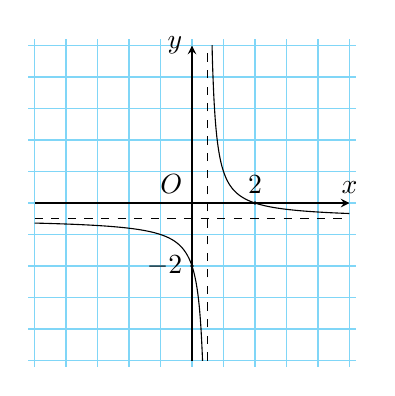
\begin{tikzpicture}[>=stealth,scale=0.4]
				\def\a{-1} 
				 \def\b{2}
				\def\c{2} 
				 \def\d{-1}
				 \draw[cyan!50,thin] (-5.2,-5.2) grid (5.2,5.2);
				\draw[->]  (-5,0) -- (5,0) node[above] {$x$};
				\draw[->] (0,-5) --  (0,5) node[left] {$y$};
				\draw (0,0) node[above left]{$O$}; 
				 \draw[dashed] (0.5,-5)--(0.5,5)
					 (-5,-0.5)--(5,-0.5);
				\clip  (-5,-5) rectangle (5,5);
				 \pgfmathsetmacro{\can}{-(\d)/(\c)}
				 \draw[samples=100,smooth,domain=-5:{\can-.1}] plot (\x,{(\a*\x+(\b))/(\c*\x+(\d))});
				\draw[samples=100,smooth,domain={\can+.1}:5] plot  (\x,{(\a*\x+(\b))/(\c*\x+(\d))});
				\draw (2,0) node[above]{$2$} circle  (1pt);
				\draw (0,-2)  node[left]{$-2$} circle (1pt);
			\end{tikzpicture}
		\end{center}
		} 
	\loigiai{ 
			\begin{itemchoice}
				\itemch Sai.  Do $f'(x)=\dfrac{-3}{(2x-1)^2}$.
				\itemch Sai. Do $f'(x)=\dfrac{-3}{(2x-1)^2}<0,  \forall x \ne \dfrac{1}{2}$.
				\itemch Sai. Hàm số đã cho  có bảng biến thiên như sau
				\begin{center}
					
\begin{tikzpicture}
						 \tkzTabInit[nocadre,lgt=1.3,espcl=3,deltacl=0.5]
						 {$x$/1,$f’(x)$/0.7,$f (x)$/2}
						{$-\infty$,$\dfrac{1}{2}$,$+\infty$} 
						 \tkzTabLine{,-,d,-,}
						\tkzTabVar{+/$-\dfrac{1}{2}$,-D+/$-\infty$/$+\infty$,-/$-\dfrac{1}{2}$} 
					\end{tikzpicture}
				\end{center}
				\itemch Đúng. Vì hàm số đã cho có đồ  thị như sau
				\begin{center}
					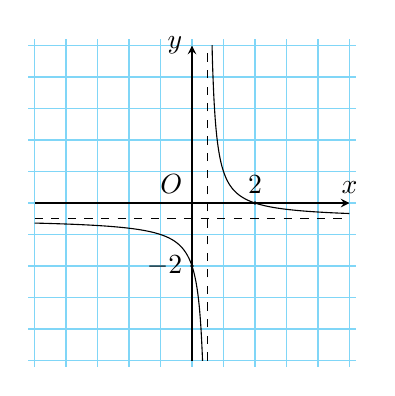
\begin{tikzpicture}[>=stealth,scale=0.4]
						 \def\a{-1}
						\def\b{2} 
						\def\c{2} 
						\def\d{-1} 
						\draw[cyan!50,thin](-5.2,-5.2) grid (5.2,5.2); 
						 \draw[->] (-5,0) -- (5,0) node[above] {$x$};
						 \draw[->] (0,-5) -- (0,5) node[left] {$y$};
						 \draw (0,0) node[above left]{$O$};
						 \draw[dashed] (0.5,-5)--(0.5,5)
						 (-5,-0.5)--(5,-0.5);
						\clip  (-5,-5) rectangle (5,5);
						\pgfmathsetmacro{\can}{-(\d)/(\c)} 
						 \draw[samples=100,smooth,domain=-5:{\can-.1}] plot (\x,{(\a*\x+(\b))/(\c*\x+(\d))});
						\draw[samples=100,smooth,domain={\can+.1}:5]  plot (\x,{(\a*\x+(\b))/(\c*\x+(\d))});
						\draw (2,0) node[above]{$2$} circle  (1pt);
						\draw (0,-2) node[left]{$-2$} circle  (1pt);
					\end{tikzpicture}
				\end{center}
			\end{itemchoice}
		 }
	\end{ex}

% nguồn: Phan1_Lop_12_Dai_so_Chuong_1
\begin{ex}%[2D1H1-1]%[ma:2e557026]
		 Cho hàm số $y=\dfrac{x^2+x-1}{x-1}$
	\choiceTF 
			{\True Tập xác định của  hàm số là $\mathscr{D}=\mathbb{R} \setminus \{1 \}$}
			{\True Phương trình  $y'=0$ có hai nghiệm nguyên}
			{Hàm số đồng biến trên mỗi khoảng  $(0;1)$ và $(2;+\infty)$}
			{\True Hàm số nghịch biến trên mỗi khoảng $(0;1)$ và $(1;2)$} 
	\loigiai{ 
			 Tập xác định $\mathscr{D} = \mathbb{R} \setminus \{1 \}$.\\
			 Ta có $y' = \dfrac{x^2-2x}{(x-1)^2} = 0 \Leftrightarrow \hoac{&x=0\\&x=2.}$
			\begin{center}
				\begin{tikzpicture}[>=stealth,scale=0.8]
					\tkzTabInit[lgt=2,espcl=2] 
						 {$x$/0.8,$y^{\prime}$/0.8,$y$/3}
						{$-\infty$,$0$,$1$,$2$,$+\infty$} 
					 \tkzTabLine{,+,0,-,d,-,0,+,}
					 \path
						 (N13) node[shift={(0,0.3)}](A){$-\infty$}
						(N22)  node[shift={(0,-0.3)}](B){$1$}
						(N33) node[shift={(-0.5,0.3)}](C){$-\infty$} 
						 (N32) node[shift={(0.5,-0.3)}](D){$+\infty$}
						(N43)  node[shift={(0,0.3)}](E){$5$}
						(N52) node[shift={(0,-0.3)}](F){$+\infty$}; 
					\foreach\X/\Y in{A/B,B/C,D/E,E/F}\draw[->](\X)--(\Y); 
					 \draw[double,double distance=2pt](N32)--(N33);
				\end{tikzpicture}
			\end{center}
			Vậy hàm số đồng  biến trên mỗi khoảng $(-\infty;0)$, $(2;+\infty)$ và nghịch biến trên mỗi khoảng $(0;1)$, $(1;2)$.
			\begin{itemchoice}
				\itemch Tập xác định của hàm số là  $\mathscr{D}=\mathbb{R} \setminus \{1 \}$.
				\itemch Phương trình $y'=0$ có hai nghiệm  nguyên.
				\itemch Hàm số đồng biến trên  mỗi khoảng $(\infty;0)$ và $(2;+\infty)$
				\itemch Hàm số nghịch biến trên mỗi khoảng $(0;1)$ và  $(1;2)$
			\end{itemchoice}
		} 
	\end{ex}

% nguồn: Phan1_Lop_12_Dai_so_Chuong_1
\begin{ex}%[2D1H1-1]%[ma:4ab27217]
		 Cho hàm số $y=\dfrac{x-1}{x+2}$.
	 \choiceTF
			{Tập xác định của  hàm số là $\mathscr{D}=\mathbb{R}$}
			{Hàm số nghịch biến trên  $\mathbb{R} \setminus \{-2 \}$}
			{Hàm số đồng  biến trên $\mathbb{R} \setminus \{-2 \}$}
			{\True Hàm số đồng biến trên các khoảng $(-\infty;-2)$ và $(-2;+\infty)$} 
	 \loigiai{
			Tập  xác định $\mathscr{D} = \mathbb{R} \setminus \{-2 \}$.\\
			 Ta có $y'=\dfrac{3}{(x+2)^2} >0$, $\forall x \in \mathbb{R} \setminus \{-2 \}$.\\
			Suy ra hàm số đồng biến trên  các khoảng $(-\infty;-2)$ và $(-2;+\infty)$.
			\begin{itemchoice}
				\itemch Tập xác định của hàm số  là $\mathscr{D}=\mathbb{R} \setminus \{-2 \}$.
				\itemch Hàm số đồng biến trên các khoảng $(-\infty;-2)$ và  $(-2;+\infty)$.
				 \itemch Hàm số đồng biến trên các khoảng $(-\infty;-2)$ và $(-2;+\infty)$.
				\itemch Hàm số đồng biến trên các khoảng $(-\infty;-2)$  và $(-2;+\infty)$.
			\end{itemchoice}
		} 
	\end{ex}

% nguồn: Phan1_Lop_12_Dai_so_Chuong_1
\begin{ex}%[2D1H1-1]%[ma:fb91a103]
		Cho hàm số $y = \dfrac{-x^2 +  2x - 1}{x + 2}$.
	\choiceTF 
			{\True Tập xác định của hàm  số là $\mathscr{D} = \mathbb{R} \setminus \{-2\}$}
			{Phương trình $y' = 0$  có hai nghiệm và hai nghiệm này là nguyên dương}
			{Hàm số đồng biến trên mỗi khoảng $(-5;  -2)$ và $(-2; +\infty)$}
			{\True Hàm số nghịch biến trên mỗi khoảng $(-\infty; -5)$  và $(1; +\infty)$}
	 \loigiai{
			\begin{itemchoice}
				\itemch Tập xác định $\mathscr{D}  = \mathbb{R} \setminus \{-2\}$.
				\itemch Đạo hàm $y' = \dfrac{-x^2 - 4x  + 5}{(x + 2)^2},\ \forall x \in \mathscr{D}$.\\
				Phương trình $y' = 0 \Leftrightarrow \dfrac{-x^2 - 4x + 5}{(x + 2)^2} = 0 \Leftrightarrow -x^2 - 4x  + 5 = 0 \Leftrightarrow \hoac{&x = 1\\&x = -5}$.\\
				Hai nghiệm không đều là nguyên dương. 
				 \itemch Bảng biến thiên
				\begin{center}
					
\begin{tikzpicture}
						\tkzTabInit[nocadre=false,lgt=1.2,espcl=2.6,deltacl=0.5] 
						 {$x$/0.7,$y'$/0.7,$y$/2.5}
						{$-\infty$,$-5$,$-2$,$1$,$+\infty$} 
						\tkzTabLine{,-,z,+,d,+,z,-,} 
						 \tkzTabVar{+/$+\infty$,-/$12$,+D-/$+\infty$/$-\infty$,+/$0$,-/$-\infty$}
					\end{tikzpicture}
				\end{center}
				Từ bảng biến thiên suy ra hàm số đồng biến trên mỗi khoảng  $(-5; -2)$ và $(-2; 1)$.
				\itemch Từ bảng biến  thiên suy ra hàm số nghịch biến trên mỗi khoảng $(-\infty; -5)$ và $(1; +\infty)$.
			\end{itemchoice}
		} 
	\end{ex}

% nguồn: Phan1_Lop_12_Dai_so_Chuong_1
\begin{ex}%[2D1H1-1]%[ma:8e9e3d8e]
		 Cho hàm số $y=f(x)=x^4-2x^2+2$
	\choiceTF 
			{Tập  xác định của hàm số $\mathscr{D}=[0;+\infty)$}
			{Hàm  số đồng biến trên khoảng $(-2;0)$}
			{\True Hàm số đồng biến trên $\left(-\dfrac{1}{2};+\infty\right)$} 
			{\True Hàm số nghịch biến  trên các khoảng $(-\infty;-1)$ và $(0;1)$}
	 \loigiai{
			Tập  xác định $\mathscr{D}=\mathbb{R}$.\\
			 Ta có $y'=4x^3-4x$. $y'=0 \Leftrightarrow 4x^3-4x=0 \Leftrightarrow \hoac{&x=0\\&x=\pm 1.}$\\
			Bảng biến thiên 
			\begin{center}
				\begin{tikzpicture}[>=stealth,scale=0.8]
					\tkzTabInit[lgt=2,espcl=2] 
						 {$x$/0.8,$y^{\prime}$/0.8,$y$/3}
						{$-\infty$,$-1$,$0$,$1$,$+\infty$} 
					 \tkzTabLine{,-,0,+,0,-,0,+,}
					 \path
						 (N12) node[shift={(0,-0.3)}](A){$+\infty$}
						(N23) node[shift={(0,0.3)}](B){$1$} 
						 (N32) node[shift={(0,-0.3)}](C){$2$}
						 (N43) node[shift={(0,0.3)}](D){$1$}
						 (N52) node[shift={(0,-0.3)}](E){$+\infty$};
					 \foreach\X/\Y in{A/B,B/C,C/D,D/E}\draw[->](\X)--(\Y);
				\end{tikzpicture}
			\end{center}
			Hàm số  đồng biến trên các khoảng $(-1;0)$ và $(1;+\infty)$, nghịch biến trên các khoảng $(-\infty;-1)$ và $(0;1)$.
			\begin{itemchoice}
				\itemch Tập xác định  của hàm số $\mathscr{D} = [0;+\infty)$.
				\itemch  Hàm số đồng biến trên khoảng $(-2;0)$.
				\itemch Hàm số đồng biến trên $\left(-\dfrac{1}{2};+\infty\right)$. 
				\itemch Hàm số  nghịch biến trên các khoảng $(-\infty;-1)$ và $(0;1)$.
			\end{itemchoice}
		} 
	\end{ex}

% nguồn: Phan1_Lop_12_Dai_so_Chuong_1
\begin{ex}%[2D1H1-1]%[ma:63ce9ed4]
		Cho hàm số $y=f(x)=x^3-3x^2-1$.  Khi đó,
	 \choiceTF
			{\True  Hàm số $y=f(x)$ có $2$ điểm cực trị}
			{\True Hàm số $y=f(x)$ đồng  biến trên $(3;+\infty)$}
			{\True Hàm số $y=f(x)$ nghịch biến  trên $(1;2)$}
			{Hàm số $y=f(x)$ đạt cực đại tại điểm $x=-3$, đạt cực tiểu tại điểm $x=-5$} 
	\loigiai{ 
			Ta có $y'=3x^2-6x$, $y'=0\Leftrightarrow 3x^2-6x=0\Leftrightarrow\hoac{&x=0\\&x=2.}$\\ 
			Bảng  biến thiên
			\begin{center}
				
\begin{tikzpicture}
					 \tkzTabInit[nocadre=false,lgt=1,espcl=2]
						 {$x$ /0.7,$y'$ /0.7,$y$ /1.7}
						{$-\infty$,$0$,$2$,$+\infty$} 
					\tkzTabLine{,+,0,-,0,+} 
					\tkzTabVar{-/$-\infty$,+/ $-3$,-/ $-5$ /,+/$+\infty$ /} 
				\end{tikzpicture}
			\end{center}
			Từ  bảng biến thiên suy ra
			\begin{itemchoice}
				 \itemch Hàm số đã cho có $2$ điểm cực trị tại $x=0$ và $x=2$.
				\itemch Vì hàm số đã cho đồng biến trên $(2;+\infty)$  nên nó đồng biến trên khoảng $(3;+\infty)$.
				\itemch Vì hàm số đã cho nghịch biến trên $(0;2)$ nên nó nghịch  biến trên khoảng $(1;2)$.
				\itemch Hàm số  đã cho có điểm cực đại tại $x=0$ và có điểm cực tiểu tại điểm $x=2$.
			\end{itemchoice}
		 }
	\end{ex}

% nguồn: Phan1_Lop_12_Dai_so_Chuong_1
\begin{ex}%[2D1H1-1]%[ma:75ab0dbe]
		Cho hàm  số $f(x)=x^3+3x^2-9x+15$.
	\choiceTF 
			{Hàm số có  đạo hàm là $f'(x)=3x^2+6x+9$}
			{Hàm số đồng biến trên khoảng  $(-3;1)$}
			{\True Khoảng nghịch biến của hàm số $f(x)$ chứa  đúng $3$ số nguyên}
			{\True Hàm số $h(x)=f(x)+\dfrac{3}{2x-x^2-4}$ đồng  biến trên $(1;+\infty)$}
	 \loigiai{
			\begin{itemchoice}
				\itemch 
				 Tập xác định $\mathscr{D}=\mathbb{R}$.\\
				Ta  có $f'(x)=3x^2+6x-9$.
				 \itemch
				$f'(x)=0\Leftrightarrow 3x^2+6x-9=0 \Leftrightarrow\left[\begin{aligned}
				&x=1\\ 
				&x=-3. 
			\end{aligned}\right.$
			\begin{center}
				
\begin{tikzpicture}
					 \tkzTabInit[nocadre=true,lgt=1.2,espcl=2.5,deltacl=0.6]
						{$x$  /0.6,$f’(x)$ /0.6,$f (x)$ /2}
						{$-\infty$,$-3$,$1$,$+\infty$} 
					 \tkzTabLine{,+,0,-,0,+,}
					\tkzTabVar{-/$-\infty$,+/$42$,-/$10$,+/$+\infty$} 
				\end{tikzpicture}
			\end{center}
			Từ bảng  biến thiên, ta thấy hàm số nghịch biến trên khoảng $(-3;1)$.
			 \itemch
			Khoảng nghịch biến của hàm số $f(x)$ chứa đúng $3$ số nguyên là  $-2;1;0$.
			 \itemch
			 Ta có $h(x)$ có tập xác định là $\mathscr{D}=\mathbb{R}$.\\
			 Dựa vào bảng biến thiên, $f(x)$ đồng biến trên $(1;+\infty)$.\\
			$g(x)=2x-x^2-4$ nghịch biến trên $(1;+\infty)$ suy ra $\dfrac{3}{g(x)}$ đồng  biến trên $(1;+\infty)$.\\
			Vậy $h(x)$ đồng  biến trên $(1;+\infty)$.
		\end{itemchoice}
	} 
\end{ex}

% nguồn: Phan1_Lop_12_Dai_so_Chuong_1
\begin{ex}%[2D1H1-1]%[ma:77dce015]
	Cho hàm số $y = x^3  - 6x^2 + 9x + 30$ có đồ thị (C).
	 \choiceTF
		{\True Hàm số xác định trên $\mathbb{R}$} 
		{\True Hàm số  đồng biến trên $(-\infty; 0)$}
		{Giá trị cực đại của hàm số bằng  30}
		{Có $5$ giá trị nguyên của $m$ để  đường thẳng $y = m$ cắt đồ thị $(C)$ tại $3$ điểm phân biệt}
	\loigiai{ 
		Tập xác định $\mathscr{D} = \mathbb{R}$.  \\
		Đạo hàm $y' =3x^2-12x+9$. 
		Cho $y'=0\Leftrightarrow \hoac{&x=1 \\ &x=3.}$  \\
		Bảng biến thiên 
		\begin{center}
			
\begin{tikzpicture}[scale=1,font=\footnotesize,line join=round,line cap=round,>=stealth]
				 \tkzTabInit[nocadre=false,lgt=1,espcl=2,deltacl=0.5]
					{$x$/.7,$y'$/.7,$y$/2} 
					 {$-\infty$,$1$,$3$,$+\infty$}
				\tkzTabLine{,+,$0$,-,$0$,+,} 
				 \tkzTabVar{-/$-\infty$,+/$34$,-/$30$,+/$+\infty$}
			\end{tikzpicture}
		\end{center}
		Từ đó, ta có 
		\begin{itemchoice}
			\itemch  Tập xác định là $\mathbb{R}$.
			\itemch Từ bảng biến thiên suy ra hàm số đồng biến trên khoảng $(-\infty; 1)$ và $(3; +\infty)$, nghịch biến trên khoảng $(1;  3)$.
			\itemch Từ bảng biến thiên suy ra giá trị cực đại  của hàm số là $f(1) = 34$.
			\itemch Đường  thẳng $y = m$ cắt $(C)$ tại $3$ điểm phân biệt khi $30<m<34$.\\
			Do $m\in  \mathbb{Z}$ nên $m\in \{31,\; 32; 33\}$. Vậy có $3$ giá trị nguyên $m$ thỏa mãn.
		\end{itemchoice}
	} 
\end{ex}

% nguồn: Phan1_Lop_12_Dai_so_Chuong_1
\begin{ex}%[2D1H1-1]%[ma:2059cb3f]
	Cho hàm số $y=f(x)$ có đồ thị như hình vẽ 
	\begin{center}
		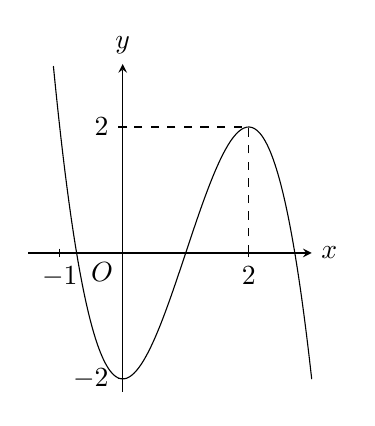
\begin{tikzpicture}[scale=0.8,>=stealth]
			\draw[->] (-1.5,0) -- (3,0)  node[right] {$x$};
			\draw[->] (0,-2.2) -- (0,3) node[above]  {$y$};
			\node[below left] at (0,0)  {$O$};
			 \foreach \x in {-1,2}
			\draw[shift={(\x,0)}]  (0pt,2pt)--(0pt,-2pt)
				node[below]  {$\x$};
			 \foreach \y in {-2,2}
			\draw[shift={(0,\y)}] (2pt,0pt) -- (-2pt,0pt) 
				node[left]  {$\y$};
			\draw[smooth,samples=100,domain=-1.1:3,font=\footnotesize,line  join=round,line cap=round]
				plot (\x,{-(\x)^3  + 3*(\x)^2 - 2});
			\draw[dashed] (2,0) -- (2,2) -- (0,2); 
		\end{tikzpicture}
	\end{center}
	 \choiceTF
		{\True  Hàm số $y=f(x)$ đồng biến trên khoảng $(0;2)$}
		{\True Hàm số $y=f(x)$ nghịch biến trên mỗi khoảng $(-\infty;0)$,  $(2;+\infty)$}
		 {\True Với mọi $x \in (0;2)$ thì hàm số $y=f(x)$ luôn nhận giá trị dương}
		 {\True Hàm số $y=f(-x)$ nghịch biến trên khoảng $(-2;0)$}
	\loigiai{ 
		Từ đồ thị, hàm số $y=f(x)$ đồng  biến trên $(0;2) \Leftrightarrow f'(x)>0 \Leftrightarrow 0<x<2$.\\
		Xét hàm  số $y=f(-x)$ có $y'=-f'(-x)$.\\
		Để hàm số nghịch biến  thì
		 \[
		y'<0 \Leftrightarrow -f'(-x)<0 \Leftrightarrow f'(-x)>0  \Leftrightarrow 0<-x<2 \Leftrightarrow -2<x<0.
		 \]
		Suy  ra hàm số $y=f(-x)$ nghịch biến trên các khoảng $(-2;0)$.
		\begin{itemchoice}
			\itemch Hàm số $y=f(x)$ đồng biến trên  khoảng $(0;2)$.
			\itemch Hàm số $y=f(x)$ nghịch biến trên mỗi khoảng $(-\infty;0)$,  $(2;+\infty)$.
			\itemch Với mọi $x \in (0;2)$ thì hàm số  $y=f(x)$ luôn nhận giá trị dương
			\itemch Hàm số $y=f(-x)$ nghịch biến  trên khoảng $(-2;0)$.
		\end{itemchoice}
	 }
\end{ex}


%%%%%%%%%%%%%%%% TRẢ LỜI NGẮN %%%%%%%%%%%%%%%%

% nguồn: Phan2_Lop_12_Dai_so_Chuong_1
\begin{bt}%[2D1H1-1]%[ma:71a91d64]
	Giả sử lợi nhuận của một cửa hàng tạp hóa nhỏ trong ngày thứ $x$ của một tháng nào đó được cho bởi công thức $h(x)=-2x^2+40x+700$ (đơn vị: nghìn đồng). Giả sử tháng đó có $30$ ngày, hỏi có bao nhiêu ngày trong tháng đó cửa hàng có lợi  nhuận tăng so với lợi nhuận ngày liền trước đó?
	\shortans{9} 
	\loigiai{ 
		Ta có  $h'(x)=-4x+40$.\\
		Khi  đó $h'(x)=0\Leftrightarrow -4x+40=0\Leftrightarrow x=10$.\\
		Bảng biến  thiên của $h(x)$ trên đoạn $[1;30]$ như sau
		\begin{center}
			
\begin{tikzpicture}
				 \tkzTabInit[nocadre=true,lgt=1.2,espcl=2.5,deltacl=0.6]{$x$/0.6,$h'(x)$/0.6,$h (x)$/2}
					 {$1$,$10$,$30$}
				\tkzTabLine {,+,0,-,} 
				\tkzTabVar{-/$738$,+/$900$,-/$100$} 
			\end{tikzpicture}
		\end{center}
		Dựa vào bảng biến thiên, ta thấy hàm lợi nhuận $h(x)$ có giá trị tăng  trên đoạn $[1;10]$.\\
		 Do đó các ngày có lợi nhuận tăng so với ngày liền trước đó là từ ngày $2$ đến ngày $10$.\\
		Vậy  có $10-2+1=9$ ngày.
	} 
\end{bt}

% nguồn: Phan2_Lop_12_Dai_so_Chuong_1
\begin{bt}%[2D1H1-1]%[ma:91d1661e]
	 Số nguyên $a$ lớn nhất để hàm số $y=\log _{\tfrac{\pi}{a}} x$ đồng biến trên khoảng $(0;+\infty)$ bằng bao nhiêu?
	\shortans{3} 
	 \loigiai{
		Để hàm số $y=\log _{\tfrac{\pi}{a}} x$ đồng biến trên khoảng $(0;+\infty)$ thì $\dfrac{\pi}{a} > 1\Leftrightarrow 0< a < \pi$.\\  Vậy số nguyên $a$ lớn nhất thỏa mãn điều kiện là $3$.
	 }
\end{bt}

% nguồn: Phan2_Lop_12_Dai_so_Chuong_1
\begin{bt}%[2D1H1-1]%[ma:592e79d8]
	Sau khi phát hiện một bệnh dịch, các chuyên gia y tế ước tính số người nhiễm bệnh kể từ ngày xuất hiện bệnh nhân đầu tiên đến ngày thứ  $t$ là $f(t)=180t+42t^2-t^3$, $t=0,1,\ldots,30$. Nếu coi $f(t)$ là hàm số xác định trên đoạn $[0;30]$ thì đạo hàm $f'(t)$ được xem là tốc độ truyền bệnh (đơn vị: người/ngày) tại thời điểm $t$. Hỏi trong $30$ ngày đó, có bao nhiêu ngày mà tốc độ truyền bệnh giảm?
	 \shortans{16}
	\loigiai{ 
		Ta có $f'(t)=180+84t-3t^2$ và $f''(t)=84-6t$.\\ 
		Khi đó  $f''(t)=0\Leftrightarrow t=14$.\\
		Bảng biến thiên của $f'(t)$ như  sau
		\begin{center}
			
\begin{tikzpicture}
				 \tkzTabInit[lgt=1.2,espcl=2.5,deltacl=0.6]{$t$/0.6,$f''(t)$/0.6,$f'(t)$/2}
					{$0$,$14$,$30$} 
				 \tkzTabLine {,+,0,-,}
				 \tkzTabVar{-/$180$,+/$768$,-/$0$}
			\end{tikzpicture}
		\end{center}
		Theo bảng biến thiên thì từ ngày thứ $15$  đến ngày thứ $30$ tốc độ truyền bệnh giảm.\\
		Vậy có $30-15+1=16$  ngày mà tốc độ truyền bệnh giảm.
	} 
\end{bt}

% nguồn: Phan2_Lop_12_Dai_so_Chuong_1
\begin{bt}%[2D1H1-1]%[ma:ebb7a220]
	Kính viễn vọng không gian Hubble được đưa vào vũ  trụ ngày $24/4/1990$ bằng tàu con thoi Discovery. Vận tốc của tàu con thoi trong sứ mệnh này, từ lúc cất cánh tại thời điểm $t=0$ s cho đến khi tên lửa đẩy được phóng đi tại thời điểm $t=26$ s được cho bởi hàm số $v(t)=0{,}001302t^3-0{,}09029t^2+23$, $v$ được tính bằng ft/s. Hỏi gia tốc của tàu con thoi sẽ tăng từ thời điểm nào tính từ lúc cất cánh cho đến khi tên lửa đẩy được phóng đi (kết quả thời gian được tính bằng giây và làm tròn đến hàng phần mười)?
	\shortans{23,1} 
	\loigiai{ 
		Gia  tốc tàu con thoi là $a(t)=v'(t)=0{,}003906t^2-0{,}18058t$.\\
		Ta có 
		 $a'(t)=0{,}007812t-0{,}18058$.\\
		Khi đó $a'(t)=0\Leftrightarrow t=\dfrac{0{,}18058}{0{,}007812}\approx  23{,}1$.\\
		Bảng  biến thiên hàm gia tốc như sau
		\begin{center}
			
\begin{tikzpicture}
				 \tkzTabInit[lgt=1.2,espcl=2.5,deltacl=0.6]{$t$/0.6,$a'(t)$/0.6,$a (t)$/2}
					 {$0$,$23{,}1$,$26$}
				\tkzTabLine  {,-,0,+,}
				 \tkzTabVar{+/,-/,+/}
			\end{tikzpicture}
		\end{center}
		Vậy kể từ thời điểm $t\approx 23{,}1$ s thì gia tốc  của tàu con thoi sẽ tăng.
	 }
\end{bt}

% nguồn: Phan2_Lop_12_Dai_so_Chuong_1
\begin{bt}%[2D1V1-1]%[ma:485fb131]
	Trong một nghiên cứu tại Viện Sức khỏe Tâm thần Quốc gia, các nhà khoa học theo dõi độ dày vỏ não (cortex) của $307$ trẻ em có IQ cao ($121-149$) qua tuổi $t$ (tính bằng năm), với mô hình $S(t) = 0{,}000989t^3 - 0{,}0486t^2  + 0{,}7116t + 1{,}46$, $5 \le t \le 19$. Hỏi vỏ não của trẻ có IQ siêu trí tuệ đạt độ dày cực đại vào khoảng bao nhiêu tuổi (\textit{làm tròn kết quả đến hàng phần trăm})?
	\shortans{11,1} 
	\loigiai{ 
		Ta có $S'(t) = 3 \cdot 0{,}000989t^2 - 2 \cdot 0{,}0486t + 0{,}7116  = 0{,}002967t^2 - 0{,}0972t + 0{,}7116$.\\
		Giải $S'(t) =  0 \Leftrightarrow 0{,}002967t^2 - 0{,}0972t + 0{,}7116 = 0$.\\
		Ta có $t = \dfrac{0{,}0972 \pm 0{,}0316}{2\cdot0{,}002967} = x \dfrac{0{,}0972 \pm 0{,}0316}{0{,}005934}  \Leftrightarrow \heva {&t_1 = \dfrac{0{,}1288}{0{,}005934} \approx 21{,}71 \quad \left(\notin [5;19]\right), \\&t_2 = \dfrac{0{,}0656}{0{,}005934} \approx 11{,}05 \quad \left(\in [5;19]\right).}$\\
		Vậy nghiệm khả  dụng duy nhất trên $[5;19]$ là $t \approx 11{,}05$.\\
		Lập bảng biến thiên hàm  số $S(t)$ suy ra $t \approx 11{,}05$ là điểm cực đại.\\
		Vậy độ  dày vỏ não của nhóm trẻ IQ cao đạt cực đại tại $t \approx 11{,}05$ tuổi.\\
	} 
\end{bt}

% nguồn: Phan2_Lop_12_Dai_so_Chuong_1
\begin{bt}%[2D1V1-1]%[ma:a23dfe64]
	Giả sử tổng  chi phí sản xuất $x$ $(0 \le x \le 50)$ đơn vị sản phẩm $A$ mỗi ngày tại một nhà máy được cho bởi công thức $C(x) = \dfrac{x^2}{4} + 3x + 400$ (nghìn đồng) và toàn bộ chúng được bán hết với giá $(900 - 6x)$ nghìn đồng một sản phẩm. Tìm mức sản lượng (đó là số lượng sản phẩm được sản xuất) để chi phí trung bình tính trên mỗi đơn vị sản phẩm là đạt cực tiểu.
	\shortans{40} 
	 \loigiai{
		Kí hiệu $\overline{C}(x)$ là chi phí trung bình tính trên mỗi đơn vị sản  phẩm.\\
		 Ta có $\overline{C}(x)=\dfrac{C(x)}{x}=\dfrac{x}{4}+3+\dfrac{400}{x}$.\\
		Đạo hàm $\overline{C'}(x)=\dfrac{x^2-1600}{4x^2}=0\Leftrightarrow x=40$ (vì $0\le x\le 50$).\\ 
		Bảng biến  thiên như sau
		\begin{center}
			\begin{tikzpicture}[scale=1]
				\tkzTabInit[nocadre=false,lgt=1.3,espcl=3,deltacl=0.6] 
					{$x$  /0.6,
					 $\overline{C'}$ /0.6
					 ,
					$\overline{C}$  /2
				} 
					{$0$,$40$,$50$} 
				\tkzTabLine{,-,0,+,} 
				\draw[->] (2.1,-1.8) node[above]{$+\infty$}--++(2.85,-0.8) coordinate (A) node[below]{$23$}; 
				\draw[->] ($(A)+(0.2,0)$)--++(2.3,0.2) node[above]{$23{,}5$}; 
				\draw[pattern = north west  lines] (1.3,0)--++(0.4,0)--++(0,-3.2)--++(-0.4,0)--cycle;
				\draw[pattern = north  west lines] (8.1,0)--++(0.4,0)--++(0,-3.2)--++(-0.4,0)--cycle;
			\end{tikzpicture}
		\end{center}
		Vậy  mức sản lượng $x=40$.
	 }
\end{bt}

% nguồn: Phan2_Lop_12_Dai_so_Chuong_1
\begin{bt}%[2D1V1-1]%[ma:5a96b368]
	Ở $45^\circ C$, phản ứng hóa học phân hủy $N_2O_5$ xảy ra theo phương trình \break$N_2O_5 \to 2NO_2 + \dfrac{1}{2}O_2$ với nồng độ $c(t)$ (mol/L) của $N_2O_5$ ($c(t)  > 0$) tại thời điểm $t$ giây ($t \ge 0$) thỏa mãn $c'(t) = -0{,}0005 \cdot c(t)$. Biết khi $t=0$, nồng độ ban đầu của $N_2O_5$ là $0{,}05$ mol/L và nồng độ trung bình của $N_2O_5$ (mol/L) từ thời điểm $a$ giây đến thời điểm $b$ giây $(a < b)$ được cho bởi công thức $\dfrac{1}{b-a} \displaystyle \int_{a}^{b} c(t) \mathrm{\,d}t$.
	Nồng độ trung bình của $N_2O_5$ từ thời điểm $10$ giây  đến thời điểm $20$ giây là $a \cdot 10^{-4}$ (mol/L). Tính $a$ (\textit{làm tròn kết quả đến hàng đơn vị}).
	\shortans{496} 
	\loigiai{ 
		Để tính  được nồng độ trung bình, ta cần tìm $c(t)$.\\
		Ta  có $c'(t) = -0{,}0005\cdot c(t)$ \\
		$\dfrac{c'(t)}{c(t)} = -0{,}0005$\\ 
		$(\ln c(t))'  = -0{,}0005$
		 Nguyên hàm 2 vế, ta được\\
		$\ln  c(t) = -0{,}0005t + C$ \\
		Suy ra  $c(t) = e^{-0{,}0005t+C}$.\\
		Cho  $t=0$ ta có $c(0)=0{,}05$ mol/L $\Rightarrow 0{,}05 = e^{C} \Rightarrow C = \ln 0{,}05$.\\
		Suy ra $c(t)  = e^{-0{,}0005t + \ln 0{,}05}$.\\
		Vì có nồng độ trung bình từ  thời điểm $10$ giây đến thời điểm $20$ giây.\\
		Nên $\dfrac{1}{b-a} \displaystyle \int_{a}^{b} c(t) \mathrm{\,d}t = \dfrac{1}{20-10} \displaystyle \int_{10}^{20} e^{-0{,}0005t + \ln 0{,}05}  \mathrm{\,d}t \approx 0{,}0496 \approx 496 \cdot 10^{-4}$.\\
		Vậy $a = 496$. 
	 }
\end{bt}

% nguồn: Phan2_Lop_12_Dai_so_Chuong_1
\begin{bt}%[2D1V1-1]%[ma:f4dd0802]
	Trọng lực của Trái Đất tác dụng  lên một vệ tinh trong quá trình vệ tinh này được phóng lên từ mặt đất tới vị trí cách tâm Trái Đất $r(m)$ xác định bởi công thức
	$F(r) = G \dfrac{Mm}{r^2}$ trong đó $M = 6 \cdot 10^{24}$ kg là khối lượng Trái Đất, $m$ (kg) là khối lượng vệ tinh và $G = 6{,}67 \cdot 10^{-11}$ N $\cdot$ m$^2$ / kg$^2$ là hằng số hấp dẫn. Trọng lực này sinh công $W = \displaystyle \int_{a}^{b} F(r) \mathrm{\,d}r$  (J) khi vệ tinh thay đổi từ vị trí cách tâm Trái Đất $a$ (m) lên vị trí cách tâm Trái Đất $b$ (m). Công tối thiểu để phóng một vệ tinh nặng $m = 1\,000$ kg từ mặt đất lên độ cao $35\,780$ km so với mặt đất là $a \cdot 10^{10}$ (J), biết bán kính Trái Đất là $6\,370$ km. Giá trị của $a$ làm tròn đến hàng đơn vị là
	\begin{center}
		\begin{tikzpicture}[line join = round,line cap=round,>=stealth,font=\footnotesize,scale=0.8]
			\draw[cyan]  (0,0) circle (1.5);
			\draw[dashed] (0,0) --++ (6.3,2.1); 
			\draw[fill=gray,line  width=1pt] (6.59,2.3) --++ (-0.17,0.25) coordinate (D) --++ (0.45,-0.15)--cycle;
			\draw[line  width=1.5pt] ($(D)+(-0.15,-0.05)$)--($(D)+(0.15,0.05)$);
			\draw[fill=gray,line width=1pt] (6.58,2.05)..controls + (190:0.05) and + (190:0.05)..++(-0.1,0.18)..controls + (120:0.05) and + (120:0.05)..++ (1.05,0.4) coordinate (A)..controls + (90:0.015) and + (90:0.015)..++  (0.35,-0.005) coordinate (B)..controls + (-30:0.01) and + (-30: 0.01)..++(-0.3,-0.23) coordinate (C)..controls + (-45:0.03) and + (-45:0.03).. cycle;
			\draw[fill=orange,line width=1pt] (A)--(B)--(C)..controls + (190:0.02) and + (190:0.02).. cycle; 
			\draw[fill=gray,line width=1pt] (6.6,2.15) --++ (0.4,0.13)..controls + (-90:0.05) and + (-70:0.05)..++(-0.57,-0.35) coordinate (E)..controls  + (0:0.05) and + (0:0.05).. cycle;
		\end{tikzpicture}
	\end{center}
	\shortans{5} 
	\loigiai{ 
		Vì công thức tính lực sinh công $W$ sẽ được tính khi vệ tinh thay đổi từ vị trí cách tâm Trái Đất $a$  (m) lên vị trí cách tâm Trái Đất $b$ (m) nên để phóng một vệ tinh lên độ cao $35\,780$ km so với mặt đất thì $b = 35\,780 + 6\,370 = 42\,150$ km $= 42\,150\,000$ m và $a = 6\,370$ km $= 6\,370\,000$ m.\\
		Ta có\\ 
		 $
		W = \displaystyle \int_{6\,370\,000}^{42\,150\,000} G \cdot \dfrac{M m}{h^2} \mathrm{\,d}h = \displaystyle \int_{6\,370\,000}^{42\,150\,000} 6{,}67 \cdot 10^{-11}  \cdot \dfrac{6 \cdot 10^{24} \cdot 1\,000}{h^2} \mathrm{\,d}h \approx 5{,}10^{10}
		$.\\ 
		 Vì công tối thiểu để phóng vệ tinh bằng công của trọng lực $W$ và bằng $5{,}10^{10}$.\\
		 Suy ra $a=5$.
	 }
\end{bt}

% nguồn: Phan2_Lop_12_Dai_so_Chuong_1
\begin{bt}%[2D1V1-1]%[ma:eaae4e6b]
	Vận tốc trung bình của dòng xe trên đoạn đường $124$ từ $6$ A.M đến $10$ A.M  được xấp xỉ bởi $f(t) = 20t - 40\sqrt{t} + 50$, $0 \le t \le 4$ trong đó $t$ tính bằng giờ kể từ $6$ A.M và $f(t)$ tính bằng km/giờ. Hỏi vào thời điểm mấy giờ trong buổi sáng (giữa $6$ A.M và $10$ A.M) thì vận tốc trung bình thấp nhất?
	 \shortans{7}
	\loigiai{ 
		Tình đạo hàm  $f'(t)=20-40 \cdot \dfrac{1}{2\sqrt{t}}=20-\dfrac{20}{\sqrt{t}}$.\\
		Xét $f'(t)=0$ ta có  $20-\dfrac{20}{\sqrt{t}}=0 \Rightarrow \dfrac{20}{\sqrt{t}}=20 \Rightarrow \sqrt{t}=1 \Rightarrow t=1$.\\
		Lập bảng xét dấu ta được\\ 
		\begin{center}
			
\begin{tikzpicture}[scale=1]
				\tkzTabInit[nocadre=false,lgt=1.2,espcl=3,deltacl=0.5] 
					{$t$ /0.6, 
					$f'(t)$ /2 
				 }
					 {$0$,$1$,$4$}
				\tkzTabLine{,-,0,+,} 
			\end{tikzpicture}
		\end{center}
		Suy ra vận tốc trung bình thấp nhất  $30$ mph xảy ra vào $7\colon00$A.M. ($t=1$).
	 }
\end{bt}

% nguồn: Phan2_Lop_12_Dai_so_Chuong_1
\begin{bt}%[2D1V1-1]%[ma:d1a9f7fd]
	Giá trị trung bình của hàm số liên tục $f(x)$  trên đoạn $[a, b]$ được định nghĩa là
	$\dfrac{1}{b-a}  \displaystyle \int_{a}^{b} f(x) \mathrm{\,d}x$.
	Giả sử nhiệt độ (tính bằng $^{\circ}\mathrm{C}$) tại thời điểm $t$ giờ trong khoảng thời gian từ $6$ giờ sáng đến $12$ giờ trưa ở một địa phương vào một ngày nào đó được mô hình hóa bởi hàm số $T(t) = 20 + 1{,}5(t-6)$, $6 \le t \le 12$. Nhiệt độ trung bình vào ngày đó trong khoảng thời gian từ $6$ giờ sáng đến  $12$ giờ trưa là bao nhiêu $^\circ C$?
	\shortans{24,5} 
	 \loigiai{
		\begin{itemize}
			 \item
			Tính tích phân của hàm số $T(t) = 20  + 1{,}5(t-6)$, $6 \le t \le 12$ từ $6$ giờ sáng đến $12$ giờ trưa.\\
			$\displaystyle \int_{6}^{12} T(t) \mathrm{\,d}t = \displaystyle \int_{6}^{12} \left[20  + 1{,}5(t-6)\right] \mathrm{\,d}t = 147$.
			\item Giá trị trung bình của hàm nhiệt độ trên khoảng từ $6$ giờ sáng đến $12$ giờ trưa là  $\dfrac{147}{12-6} = 24{,}5$.
			\item Như vậy nhiệt độ trung bình  vào ngày đó trong khoảng thời gian từ $6$ giờ sáng đến $12$ giờ trưa là $24{,}5^{\circ}$.
		\end{itemize}
	 }
\end{bt}

% nguồn: Phan2_Lop_12_Dai_so_Chuong_1
\begin{bt}%[2D1V1-1]%[ma:02e4393d]
	Một bể nước hình nón tròn xoay như hình vẽ có chiều cao $10$ m và bán kính đáy $4$ m được đổ nước đến độ cao $8$ m. Công để bơm hết nước ra từ một vòi ở đỉnh bể được tính theo  công thức $W = 9{,}8 \cdot\displaystyle \int_{2}^{10}x\cdot S(x) \mathrm{\,d}x$ (đơn vị kilôJun), trong đó $S(x)$ (m$^2$) là diện tích của lớp nước cách mặt bể $x$ m. Tính $W$ (kJ) (\textit{kết quả làm tròn đến hàng đơn vị}).
	\begin{center}
		\begin{tikzpicture}[line join = round,line cap=round,>=stealth,font=\footnotesize,scale=1.2]
			\draw[fill=cyan,opacity=0.4] (0,5) coordinate (A) arc (180:0:2cm and 0.45cm) coordinate  (B) arc (0:-180:2cm and 0.45cm);
			\draw[fill=cyan,opacity=0.6] ($(A)!1/3!(2,0)$) coordinate (D) arc  (180:0:1.325cm and 0.3cm) coordinate (E) arc (0:-180:1.325cm and 0.3cm);
			\draw[fill=cyan!50!blue]  ($(A)!2/3!(2,0)$) coordinate (P) arc (180:0:0.66cm and 0.1cm) coordinate (P1) arc (0:-180:0.66cm and 0.1cm);
			\draw[fill=cyan,opacity=0.4] (A) -- (2,0)  -- (B) arc (0:-180:2cm and 0.45cm);
			\draw[fill=cyan,opacity=0.6] (D) --  (2,0) -- (E) arc (0:-180:1.325cm and 0.3cm);
			 \draw[<->] (2.1,0) --++ (1.9,0) node[midway,above]{$4$ m};
			\draw[<->] (4.1,0.1) --++ (0,4.9)  node[midway,right]{$10$ m};
			\draw[<->] (0,0) --++ (0,3.2) node[midway,left]{$8$ m}; 
			\draw ($(P)!1/2!(P1)$)  node{\tiny$S (x)$};
		\end{tikzpicture}
	\end{center}
	\shortans{3363} 
	 \loigiai{
		Để tính được công để bơm hết nước ra thì ta cần đi tìm  hàm $S(x)$.\\
		Lớp nước cách mặt bể là một hình  tròn song song và cách mặt bể $x$ (m). Giả sử lớp nước hình tròn đó có bán kính là $r$ (m). Ta gắn trục tọa độ như hình sau.
		\begin{center}
			\begin{tikzpicture}[line join = round,line cap=round,>=stealth,font=\footnotesize,scale=0.7]
				 \def\xmin{0}; \def\xmax{13}; \def\ymin{0}; \def\ymax{7}
				\draw[->,red]  (\xmin,3)--(\xmax,3) node[below]{$x$};
				 \draw[->,red] (2,\ymin)--(2,\ymax) node[left]{$y$};
				\path 
					(2,3)  coordinate (O)
					 (2,5.5) coordinate (B)
					 (2,0.5) coordinate (B')
					(12,3)  coordinate (A)
					($(B)!2/3!(A)$) coordinate (D) 
					 ($(O)!2/3!(A)$) coordinate (C);
				\foreach \p/\r  in {B/160,O/-135,A/-90,D/90,C/-120}
				\fill (\p) circle (1.2pt)  node[shift={(\r:3mm)}]{$\p$};
				\draw (B) arc  (90+360:-90:1cm and 2.5cm);
				\draw  (B)--(A)--(B');
				\draw ($(B')!1/3!(A)$) arc (-90:90+360:0.6cm  and 1.66cm);
				\draw (D)  arc (90+360:-90:0.3cm and 0.835cm);
				\draw[dashed] (D)--($(B')!2/3!(A)$); 
			\end{tikzpicture}
		\end{center}
		Từ giả thiết,  ta có $OC = x \Rightarrow AC=10-x$; $OA=10$; $OB=4$.\\
		Vì mặt nước cách bể song song  với mặt bể .\\
		Nên  $CD \parallel OB$.\\
		Xét $\triangle OAB$ có $CD \parallel OB$  (cmt)\\
		Suy ra  $\dfrac{AC}{OA}=\dfrac{CD}{OB}$ (hệ quả Thales)\\
		$\dfrac{10-x}{10} =  \dfrac{r}{4}$\\
		Suy ra $r=\dfrac{4(10-x)}{10}=\dfrac{20-2x}{5}$.\\ 
		Do đó $S(x)=\pi  r^2=\pi\left(\dfrac{20-2x}{5}\right)^2$.\\
		Vậy $W = 9{,}8 \displaystyle \int_{2}^{10} x \cdot \pi \left( \dfrac{20-2x}{5} \right)^2 \mathrm{\,d}x \approx 3363$ (kJ). 
	 }
\end{bt}

% nguồn: Phan2_Lop_12_Dai_so_Chuong_1
\begin{bt}%[2D1V1-1]%[ma:1db93ce4]
	Lợi nhuận tổng hàng ngày (tính theo đô la) mà TKK Corporation  thu được từ việc sản xuất và bán $x$ đĩa DVD có thể ghi lại được cho bởi hàm lợi nhuận $P(x)=-0,000001x^3+0,001x^2+5x-500$; $0 \le x \le 2000$.\\
	Tìm mức sản xuất $x$ để lợi nhuận hàng ngày  đạt cực đại. (\textit{làm tròn kết quả đến hàng đơn vị}).
	\shortans{1667} 
	 \loigiai{
		Tính đạo hàm $P(x)\colon$ $P'(x)=\left(-10^{-6}x^3+10^{-3}x^2+5x-500\right)'=-3\cdot  10^{-6}x^2+2\cdot 10^{-3}x+5$.\\
		Xét $P'(x)=0$  ta có $-3\cdot 10^{-6}x^2+0{,}002x+5=0\Rightarrow 3\cdot 10^{-6}x^2-0{,}002x-5=0$.\\
		Chia  cả hai vế cho $10^{-6}$ ta có $3x^2-2\,000x-5\,000\,000=0$.\\
		Giải phương trình bậc hai: 
		\begin{align*}
			x&=\dfrac{2\,000\pm\sqrt{2\,000^2+4\cdot 3\cdot  5\,000\,000}}{2\cdot 3}=\dfrac{2\,000\pm\sqrt{4\,000\,000+60\,000\,000}}{6}
			 &=\dfrac{2\,000\pm\sqrt{64\,000\,000}}{6}=\dfrac{2\,000\pm 8\,000}{6}.
		\end{align*}
		Kết quả $x_1=\dfrac{2\,000+8\,000}{6}=\dfrac{10\,000}{6}\approx 1\,666{,}67$, $x_2=\dfrac{2\,000-8\,000}{6}=-1\,000$ (loại).\\ 
		Chọn $x=1\,666{,}67$  (nằm trong đoạn $[0;2\,000]$).\\
		Lập bảng biến thiên  ta suy ra được $P$ đạt cực đại tại $x\approx 1666,67$.\\
		Để lợi nhuận hàng ngày lớn  nhất, TKK Corporation nên sản xuất khoảng $1667$ DVD.
	 }
\end{bt}

% nguồn: Phan2_Lop_12_Dai_so_Chuong_1
\begin{bt}%[2D1V1-1]%[ma:dc3ad6a3]
	Trong một  phản ứng hóa học, tốc độ phản ứng $v$ được biểu diễn theo công thức: $v=k\cdot[A]^2\cdot[B]$, trong đó
	\begin{itemize}
		 \item $v$ là tốc độ phản ứng (mol/l/s),
		\item $k=0{,}1$ là hằng số tốc  độ phản ứng,
		\item $[A]$ và $[B]$ lần lượt là nồng độ của hai chất  phản ứng (mol/l).
	\end{itemize}
	Giả sử tổng nồng độ ban đầu của $[A]$ và $[B]$ là $C=2$ mol/l, tức là $[A]+[B]=2$. Hãy tìm  nồng độ của $[A]$ tại đó tốc độ phản ứng $v$ đạt cực đại. (kết quả làm tròn đến hàng phần trăm)
	\shortans{1,33} 
	\loigiai{ 
		Ta có $[B]=2-[A]$ nên $v=0{,}1\cdot[A]^2\cdot\left(2-[A]\right)=0{,}1\cdot\left(2[A]^2-[A]^3\right)$ với $0\le  [A]\le 2$.\\
		Đạo  hàm của $v$ theo $[A]$ là $v'=0{,}1\cdot\left(4[A]-3[A]^2\right)$.\\
		$v'=0\Leftrightarrow[A]=0$ hoặc $[A]=\dfrac{4}{3}$. 
		\begin{itemize}
			\item Với $[A]=0$ tốc độ phản ứng $v=0$ (loại vì  không có ý nghĩa thực tế).
			\item Với $[A]=\dfrac{4}{3}$ thì $v=\dfrac{16}{135}$ (mol/l/s),  đây là giá trị hợp lý.
		\end{itemize}
		Kết luận:  Với $[A]=\dfrac{4}{3}\approx 1{,}33$ (mol/l) thì tốc độ phản ứng $v$ đạt cực đại.
	} 
\end{bt}

% nguồn: Phan2_Lop_12_Dai_so_Chuong_1
\begin{bt}%[2D1V1-1]%[ma:cb92c2df]
	Hiệu suất của tim là lưu lượng máu được bơm bởi tim trên một đơn vị thời gian (lưu lượng máu chảy vào động mạch chủ). Để đo hiệu suất của tim, người ta bơm $A$ (mg) chất chỉ thị màu vào tâm nhĩ phải, chảy qua  tim rồi vào động mạch chủ và đo nồng độ chất chỉ thị màu còn lại ở tim đến thời điểm $T(s)$ khi chất chỉ thị màu tan sạch. Gọi $c(t)$ là nồng độ (mg/l) chất chỉ thị màu tại thời điểm $t(s)$ thì hiệu suất của tim được xác định bởi
	$F = \dfrac{A}{\displaystyle \int_{0}^{T} c(t) \mathrm{\,d}t}$ (I/s). 
	Biết $c(t)=\dfrac{1}{4}t(12-t)$ với $0 \le t \le 12$. Tính hiệu suất của tim khi bơm $8$ mg chất  chỉ thị màu vào tâm nhĩ phải (\textit{làm tròn đến hàng phần trăm theo đơn vị $l/s$}).
	\shortans{0,11} 
	 \loigiai{
		Tóm tắt đề bài: 
		\begin{itemize}
			\item $A = 8$ mg  (lượng chất chỉ thị màu được bơm vào).
			\item $c(t) = \dfrac{1}{4} t (12 -  t)$ với $0 \le t \le 12$.
			\item $T$ là thời điểm chất chỉ thị màu tan sạch nên $c(T) = 0$. 
		\end{itemize}
		Cho 
		\begin{eqnarray*}
			c(t) = &\dfrac{1}{4} t (12 - t)& =  0\\
			t = 0 &\text{ hoặc}& t = 12. 
		\end{eqnarray*}
		Vì $T$ là thời điểm chất chỉ thị màu tan sạch (sau khi  bơm) nên $T = 12$ giây.\\
		 Vậy ta cần tính $\displaystyle \int_{0}^{12} \dfrac{1}{4} t (12 - t) dt$.
		\begin{eqnarray*}
			\displaystyle \int_{0}^{12} \dfrac{1}{4} \left(12t - t^2\right) dt  &=& \dfrac{1}{4} \displaystyle \int_{0}^{12} \left(12t - t^2\right) \mathrm{\,d}t \\
			&=& \dfrac{1}{4} \left.\left[12 \dfrac{t^2}{2} -  \dfrac{t^3}{3} \right]\right|_{0}^{12} \\
			&=& \dfrac{1}{4} \left.\left[6t^2 - \dfrac{t^3}{3}  \right]\right|_{0}^{12} \\
			&=& \dfrac{1}{4} \left[\left( 6\cdot12^2 - \dfrac{12^3}{3} \right) - \left( 6\cdot0^2  - \dfrac{0^3}{3} \right) \right] \\
			&=&  \dfrac{1}{4} \left( 6\cdot144 - \dfrac{1728}{3} - 0 \right) \\
			&=& 72. 
		\end{eqnarray*}
		Tính hiệu suất của  tim $F$
		\begin{eqnarray*}
			F &=& \dfrac{A}{\displaystyle \int_{0}^{T} c(t) \mathrm{\,d}t}\\ 
			 &=& \dfrac{8}{72} \\
			&=&  \dfrac{1}{9}\\
			&=&0{,11} \  (I/s).
		\end{eqnarray*}
	 }
\end{bt}

% nguồn: Phan2_Lop_12_Dai_so_Chuong_1
\begin{bt}%[2D1C1-1]%[ma:71644fd2]
	Gọi $(P)$ là parabol qua $3$ điểm cực trị của đồ thị hàm số $y=\dfrac{1}{4}x^4-mx^2+m^2$.  Tìm tất cả các giá trị thực của tham số $m$ để $(P)$ qua $A(2;24)$.
	\shortans{6} 
	 \loigiai{$y'=x^3-2mx$, $y'=0\Leftrightarrow\hoac{&x=0\\
		 &x^2=2m.}$\\
		Để đồ thị hàm số có ba cực trị thì $m  > 0$.\\
		$y'=0\Leftrightarrow\hoac{ &x=0\Rightarrow y=m^2\\ 
		&x=\pm\sqrt{2m}\Rightarrow  y=0.}$\\
		Vậy ba điểm cực trị của đồ thị hàm số là $A(0;m^2)$, $B(\sqrt{2m};0)$, $C(-\sqrt{2m};0)$.\\ 
		Gọi $(P)\colon y=ax^2+bx+c$ là parabol qua  ba cực trị của đồ thị hàm số.\\
		 $\Rightarrow\heva{&c=m^2\\
		 &2ma+b\sqrt{2m}+c=0\\
		&2ma-b\sqrt{2m}+c=0}\Leftrightarrow\heva{&c=m^2\\ 
		&a=-\dfrac{m}{2}\\ 
		&b=0}\Rightarrow y=-\dfrac{m}{2}x^2+m^2$.\\ 
		Để $(P)$ đi  qua $A(2;24)$ thì $24=-\dfrac{m}{2}\cdot4+m^2\Leftrightarrow m^2-2m-24=0\Leftrightarrow\hoac{&m=6\\
		&m=-4.}$  \\
		Do $m > 0$  nên nhận $m=6$.
	} 
\end{bt}


%%%%%%%%%%%%%%%% TỰ LUẬN %%%%%%%%%%%%%%%%

% nguồn: Phan2_Lop_12_Dai_so_Chuong_1
\begin{bt}%[2D1H1-1]%[ma:e136caa3]
	Xét tính đơn  điệu của hàm số $y=4x^3+3x^2-36x+6$.
	\loigiai{ 
		Tập xác định $\mathscr{D}=\mathbb{R}$, 
		 $y'=12x^2+6x-36$.
		 Cho $y'=0$ $\Rightarrow \hoac{&{x=-2} \\&{x=\dfrac{3}{2}}.}$\\
		Bảng  biến thiên
		\begin{center}
			
\begin{tikzpicture}[>=stealth,scale=1]
				 \tkzTabInit[lgt=2,espcl=2.5,deltacl=0.8]
					 {$x$/.8,$f'(x)$/.8,$f (x)$/2}
					 {$-\infty$,$-2$,$\dfrac{3}{2}$,$+\infty$}
				\tkzTabLine{,+,0,-,0,+,} 
				 \tkzTabVar{-/$-\infty $,+/$58$,-/$-\dfrac{111}{4}$,+/$+\infty$}
			\end{tikzpicture}
		\end{center}
		Từ bảng biến thiên suy  ra\\
		Hàm số đồng biến trên khoảng $(-\infty;-2)$  và $\left(\dfrac{3}{2};+\infty \right)$.\\
		Hàm số nghịch biến trên khoảng  $\left(-2; \dfrac{3}{2} \right)$.
	} 
\end{bt}

% nguồn: Phan2_Lop_12_Dai_so_Chuong_1
\begin{bt}%[2D1H1-1]%[ma:ef69256c]
	Tìm tất cả các giá trị của tham số $m$  để các hàm số
	\begin{enumerate}[a)]
		\item $y=x^3+mx^2+2mx+2$  đồng biến trên $\mathbb{R}$.
		\item $y=-\dfrac{1}{3}x^3-mx^2+(2m-3)x-m+2$  nghịch biến trên $\mathbb{R}$.
		\item $y=-\dfrac{1}{3}x^3-mx^2+(2m+1)x+1$ nghịch biến trên khoảng $(0;5)$. 
		 \item $y=x^3-3x^2+(5-m)x$ đồng biến trên khoảng $(2;+\infty)$.
		\item  $y=\dfrac{x^3}{3}+\dfrac{mx^2}{2}+x+6$ đồng biến trên nửa khoảng $[1;+\infty)$.
		\item  $y=-x^3-6x^2+(4m-9)x+4$ nghịch biến trên khoảng $(-\infty;-3)$.
		 \item $y=x^3+mx^2+m$ nghịch biến trên $(0;2)$.
		\item $y=(m-1)x^3-3(m-1)x^2+3x+2$ đồng biến trên $\mathbb{R}$. 
	\end{enumerate}
	 \loigiai{
		\begin{enumerate}[a)]
			\item  $y=x^3+mx^2+2mx+2$ đồng biến trên $\mathbb{R}$\\
			Tập xác định $\mathscr{D}=\mathbb{R}$ và có  đạo hàm $y'=3x^2+2mx+2m$.\\
			Hàm số đã cho đồng biến trên $\mathbb{R}$ khi  và chỉ khi
			\[ 
			y'\geq 0,~\forall x \in \mathbb{R} \Leftrightarrow m^2-6m \leq 0 \Leftrightarrow 0  \leq m \leq 6.
			\] 
			\item $y=-\dfrac{1}{3}x^3-mx^2+(2m-3)x-m+2$ nghịch  biến trên $\mathbb{R}$\\
			Tập xác  định $\mathscr{D}=\mathbb{R}$ và có đạo hàm $y'=-x^2-2mx+2m-3$.\\
			Hàm số đã cho nghịch biến  trên $\mathbb{R}$ khi và chỉ khi
			\[ 
			y'\leq 0,~\forall x \in \mathbb{R} \Leftrightarrow m^2+2m-3 \leq 0 \Leftrightarrow -3 \leq m \leq  1.
			 \]
			\item $y=-\dfrac{1}{3}x^3-mx^2+(2m+1)x+1$  nghịch biến trên khoảng $(0;5)$\\
			Tập  xác định $\mathscr{D}=\mathbb{R}$ và có đạo hàm $y'=x^2-2mx+(2m+1)=0 \Leftrightarrow \hoac{&x=-1\\&x=2m+1.}$\\
			Nếu $2m+1\leq -1\Leftrightarrow m \leq -1$ thì $y' \leq 0  \Leftrightarrow x \in [2m+1;1]$ nên hàm số không nghịch biến trên khoảng $(0;5)$ nên $m \leq -1$ không thỏa mãn.\\
			Nếu $2m+1 >-1  \Leftrightarrow m>-1$ thì $y' \leq 0 \Leftrightarrow x \in [-1;2m+1]$.\\
			Để hàm số nghịch biến trên khoảng $(0;5)$  thì ta có $2m+1 \geq 5 \Leftrightarrow m \geq 2$.
			\item $y=x^3-3x^2+(5-m)x$ đồng  biến trên khoảng $(2;+\infty)$\\
			Tập xác định $\mathscr{D}=\mathbb{R}$ và  có đạo hàm $y'=3x^2-6x+5-m$.\\
			Hàm số đồng biến trên khoảng $(2;+\infty)$ khi và chỉ khi 
			\[ 
			y'\geq 0,~\forall x\in (2;+\infty)  \Leftrightarrow
			x^3-3x^2+(5-m)x \geq  0,~\forall x\in (2;+\infty)
			\Leftrightarrow  m \leq 3x^2-6x+5,~\forall x \in (2;+\infty)
			 \]
			 Xét hàm số $g(x) = 3x^2-6x+5$ trên $(2;+\infty)$ có $g'(x)=6x-6=0 \Leftrightarrow x=1$.\\
			Bảng biến thiên  của $g(x)$
			\begin{center}
				\begin{tikzpicture}[>=stealth,scale=0.7]
					 \tkzTabInit[lgt=2,espcl=6]
						{$x$/0.8,$g^{\prime} 
						(x)$/0.8,$g (x)$/3} 
						 {$2$,$+\infty$}
					\tkzTabLine{,+,} 
					 \path
						 (N13) node[shift={(0,0.3)}](A){$5$}
						(N22)  node[shift={(0,-0.3)}](B){$+\infty$};
					 \foreach\X/\Y in{A/B}\draw[->](\X)--(\Y);
				\end{tikzpicture}
			\end{center}
			Dựa vào bảng biến thiên của $g(x)$ ta được $m \leq 3x^2-6x+5$, $\forall x \in  (2;+\infty) \Leftrightarrow m \leq 5$.
			\item  $y=\dfrac{x^3}{3}+\dfrac{mx^2}{2}+x+6$ đồng biến trên nửa khoảng $[1;+\infty)$\\
			Tập xác định $\mathscr{D}=\mathbb{R}$ và có đạo hàm $y'=x^2+mx+1$.\\ 
			Hàm số đồng biến trên nửa khoảng $[1;+\infty)$  khi và chỉ khi
			\[ 
			 y'\geq 0,~\forall x \in [1;+\infty) \Leftrightarrow
			x^2+mx+1 \geq 0,~\forall x \in [1;+\infty) 
			\Leftrightarrow m \geq -x-\dfrac{1}{x},~\forall x \in  [1;+\infty).
			\] 
			Xét hàm số $g(x)=-x-\dfrac{1}{x}$ trên nửa khoảng $[1;+\infty)$ có $g'(x) =  -1 + \dfrac{1}{x^2} = \dfrac{1-x^2}{x^2}$\\
			$g'(x)=0  \Leftrightarrow \hoac{&x=1\\&x=-1.}$\\
			Bảng biến thiên của hàm số  $g(x)$ trên nửa khoảng $[1;+\infty)$
			\begin{center}
				\begin{tikzpicture}[>=stealth,scale=1]
					 \tkzTabInit[lgt=2,espcl=6]
						{$x$/0.8,$g^{\prime} 
						(x)$/0.8,$g  (x)$/3}
						 {$1$,$+\infty$}
					 \tkzTabLine{0,-,}
					 \path
						(N12)  node[shift={(0,-0.3)}](A){$-2$}
						(N23) node[shift={(0,0.3)}](B){$-\infty$}; 
					 \foreach\X/\Y in{A/B}\draw[->](\X)--(\Y);
				\end{tikzpicture}
			\end{center}
			Từ bảng biến thiên $m \geq -x-\dfrac{1}{x}$, $\forall x \in [1;+\infty)  \Leftrightarrow m \geq -2$.
			\item $y=-x^3-6x^2+(4m-9)x+4$ nghịch biến  trên khoảng $(-\infty;-3)$\\
			Tập xác định $\mathscr{D}=\mathbb{R}$ và  có đạo hàm $y'=-3x^2-12x+4m-9$.\\
			Hàm số nghịch biến trên khoảng  $(-\infty;-3)$ khi
			 \[
			y' \leq 0,~\forall x\in  (-\infty;-3) \Leftrightarrow
			 -3x^2-12x+4m-9 \leq 0,~\forall x \in (-\infty;-3)
			\Leftrightarrow 4m \leq 3x^2+12x+9,~\forall x  \in (-\infty;-3).
			\] 
			Đặt $f(x)=3x^2+12x+9$  có $f'(x)=6x+12=0 \Leftrightarrow x=-2$.\\
			Ta có bảng biến thiên của  $f(x)$
			\begin{center}
				\begin{tikzpicture}[>=stealth,scale=1]
					\tkzTabInit[lgt=2,espcl=2.7] 
						 {$x$/0.8,$g^{\prime}
						(x)$/0.8,$g (x)$/3} 
						 {$-\infty$,$-3$,$-2$,$+\infty$}
					\tkzTabLine{,-,1,-,0,+,} 
					 \path
						(N12)  node[shift={(0,-0.3)}](A){$+\infty$}
						 (N22) node[shift={(0,-1.5)}](B){$ $}
						(N33) node[shift={(0,0.3)}](C){$-3$} 
						(N42) node[shift={(0,-0.3)}](D){$+\infty$}; 
					\foreach\X/\Y  in{A/B,B/C,C/D}\draw[->](\X)--(\Y);
				\end{tikzpicture}
			\end{center}
			Dựa vào bảng biến thiên ta  thấy $4m \leq 3x^2+12x+2$, $\forall x \in (-\infty;-3)
			\Leftrightarrow 4m  \leq 0 \Leftrightarrow m \leq 0$.\\
			Vậy $m\leq 0$ hàm số nghịch biến  trên khoảng $(-\infty;-3)$.
			\item $y=x^3+mx^2+m$ nghịch biến trên  $(0;2)$\\
			 Tập xác định $\mathscr{D}=\mathbb{R}$ và có đạo hàm $y'=3x^2+2mx$.\\
			 Hàm số nghịch biến trên $(0;2)$ khi và chỉ khi
			\[ 
			y' \leq 0,~\forall x \in (0;2) \Leftrightarrow 3x^2+2mx \leq 0,~\forall x \in (0;2) \Leftrightarrow 
			m  \leq -\dfrac{3}{2}x,~\forall x \in (0;2).
			 \]
			Xét hàm số  $y=-\dfrac{3}{2}x$ trên khoảng $(0;2)$, ta có bảng biến thiên
			\begin{center}
				\begin{tikzpicture}[>=stealth,scale=1]
					\tkzTabInit[lgt=2,espcl=6] 
						{$x$/0.8,$g^{\prime} 
						(x)$/0.8,$g (x)$/3} 
						{$0$,$2$} 
					 \tkzTabLine{,-,}
					\path 
						(N12) node[shift={(0,-0.3)}](A){$0$} 
						(N23) node[shift={(0,0.3)}](B){$-3$}; 
					 \foreach\X/\Y in{A/B}\draw[->](\X)--(\Y);
				\end{tikzpicture}
			\end{center}
			Vậy để hàm số nghịch  biến trên $(0;2)$ thì $m \leq -3$.
			\item $y=(m-1)x^3-3(m-1)x^2+3x+2$ đồng biến trên $\mathbb{R}$\\ 
			Tập xác định  $\mathscr{D}=\mathbb{R}$ và có đạo hàm $y'=3(m-1)x^2-6(m-1)x+3$.\\
			Hàm số  đã cho đồng biến trên $\mathbb{R}$ khi và chỉ khi
			\[ 
			y'  \geq 0,~\forall x\in \mathbb{R}
			\Leftrightarrow \hoac{&m-1=0\\&\heva{&m-1>0\\&\Delta' \leq 0}} 
			\Leftrightarrow \hoac{&m=1\\&\heva{&m>1\\&1 \leq m \leq 2}} 
			\Leftrightarrow 1 \leq m  \leq 2.
			\] 
		\end{enumerate}
	} 
\end{bt}

% nguồn: Phan2_Lop_12_Dai_so_Chuong_1
\begin{bt}%[2D1H1-1]%[ma:61a11692]
	Tìm các khoảng đồng biến, nghịch biến của các hàm  số sau:
	\begin{enumEX}{2}
		\item  $y=\sqrt{x^2-6x+5}$.
		\item  $y=\dfrac{5x+9}{x-1}$.
		 \item $y=(x-2)\left(x^2+1\right)$.
		\item  $y=\dfrac{x^2+2x+2}{x+1}$.
	\end{enumEX}
	 \loigiai{
		\begin{enumEX}{1}
			\item Tập xác định  $ \mathscr{D}= (-\infty;1]\cup [5;+\infty)$.\\
			Ta có $ y' = \dfrac{x - 3}{\sqrt{x^2 - 6x + 5}} $; $y'=0\Leftrightarrow x-3=0\Leftrightarrow  x=3\notin \mathscr{D}$. Ta có bảng biến thiên
			\begin{center}
				
\begin{tikzpicture}[scale=1]
					\tikzset{h style/.style  ={pattern=north west lines}}
					\tkzTabInit[lgt=1.5,espcl=2.5]{$x$ /1,$y'$  /1,$y$ /2}
						{$-\infty$,$ 1 $,$ 5 $,$+\infty$} 
					\tkzTabLine{,-,d,h,d,+,} 
					\tkzTabVar{+/$+\infty$,-H/$0$,-/$0$,+/$+\infty  $}
				\end{tikzpicture}
			\end{center}
			Ta thấy hàm số đồng  biến trên $ (5; + \infty) $.
			 \item Tập xác định của hàm số $\mathscr{D}=\mathbb{R}\setminus\{1\}$.\\
			Do $y'=\dfrac{(5x+9)'(x-1)-(x-1)'(5x+9)}{(x-1)^2}=-\dfrac{14}{(x-1)^2}<0,\,\forall x\in\mathscr{D}$ suy ra hàm số nghịch biến  trên các khoảng $(-\infty;1)$ và $(1,+\infty)$.
			\item Ta có $y=x^3-2x^2+x-2$, tập xác định $\mathscr{D}=\mathbb{R}$. Đạo  hàm
			$y'=3x^2-4x+1$.\\ 
			Giải phương trình $y'=0  \Leftrightarrow \hoac{&x=1\\&x=\dfrac{1}{3}.}$\\
			Ta có bảng xét dấu  của đạo hàm.
			\begin{center}
				
\begin{tikzpicture}[>=stealth,scale=1]
					\tkzTabInit[nocadre=false,lgt=1.2,espcl=2.5,deltacl=0.6] 
						{$x$ /1,$y’$ /0.8} 
						 {$-\infty$,$\dfrac{1}{3}$,$1$,$+\infty$}
					 \tkzTabLine{,+,z,-,z,+,}
				\end{tikzpicture}
			\end{center}
			Từ bảng xét dấu đạo hàm ta thấy hàm số  nghịch biến trên khoảng $\left(\dfrac{1}{3};1\right)$ và đồng biến trên các khoảng $\left(-\infty;\dfrac{1}{3}\right)$ và $(1;+\infty)$.
			\item \begin{itemize}
			\item Tập xác định  $\mathscr{D}=\mathbb{R}\setminus \left\{-1\right\}$.
			\item $y'=\dfrac{x^2+2x}{(x+1)^2}$, $y'=0\Leftrightarrow \hoac{&  x=-2 \\ & x=0.}$\\
			Ta có  bảng biến thiên
			\begin{center}
				
\begin{tikzpicture}
					\tkzTabInit[nocadre=false,lgt=1,espcl=2] 
						 {$x$ /0.7,$y'$ /0.7,$y$ /2}
						 {$-\infty$,$-2$,$-1$,$0$,$+\infty$}
					\tkzTabLine{,+,$0$,-,d,-,$0$,+,} 
					\tkzTabVar{-/$-\infty$,+/$-2$,-D+/$-\infty$/$+\infty$,-/$2$,+/$+\infty$} 
				\end{tikzpicture}
			\end{center}
			Hàm số đồng biến trên khoảng  $\left( -\infty;-2\right)$ và $\left( 0;+\infty\right)$; nghịch biến trên $(-2;-1)$ và $(-1;0)$.
		\end{itemize}
	\end{enumEX}
 }
\end{bt}

% nguồn: Phan2_Lop_12_Dai_so_Chuong_1
\begin{bt}%[2D1H1-1]%[ma:92604a4c]
	Xét tính đơn điệu của hàm  số $y=\sqrt{-x^2+4}$.
	\loigiai{ 
		Điều kiện $-x^2+4\ge 0\Leftrightarrow-2\le  x\le 2$.\\
		 Tập xác định $\mathscr{D}=[-2; 2]$,
		 $y'=\dfrac{-x}{\sqrt{-x^2+4}}$.\\
		Cho $y'=0$ $\Rightarrow  x=0$.\\
		\begin{center}
			
\begin{tikzpicture}
				 \tkzTabInit[nocadre=false,lgt=1.5,espcl=2,deltacl=0.6]
					 {$x$/0.7,$f'(x)$/0.7,$f (x)$/2}
					{$-\infty$,$-2$,$0$,$2$,$+\infty$} 
				 \tkzTabLine{,h,d,+,$0$,-,d,h,}
				 \tkzTabVar{+H/,-/$0$,+/$2$,-H/$0$,}
			\end{tikzpicture}
		\end{center}
		 Hàm số đồng biến trên khoảng $(-2; 0)$.\\
		Hàm số nghịch biến trên khoảng $(0;  2)$.
	} 
\end{bt}
